\documentclass[12pt,a4paper]{article} % Dropped to 10pt font
\usepackage[margin=2.5cm]{geometry}   % Shaved a full cm off every margin
%% ── Packages ────────────────────────────────────────────────────────────────
\usepackage{amsmath,amssymb}
\usepackage{booktabs}
\usepackage{graphicx}
\usepackage{subcaption}
\usepackage{hyperref}
\usepackage{xcolor}
\usepackage{listings}
\usepackage{float}
\usepackage{enumitem}
\usepackage{multirow}
\usepackage{array}
\usepackage{parskip}
\usepackage{titlesec}
\usepackage{fancyhdr}
\usepackage{caption}
\usepackage[expansion=false]{microtype}

% ── Spacing compression ──────────────────────────────────────────────────────
\captionsetup{font=footnotesize,skip=2pt}
\setlist{nosep,topsep=1pt,partopsep=0pt}
\titlespacing*{\section}{0pt}{5pt plus 2pt minus 2pt}{2pt plus 1pt}
\titlespacing*{\subsection}{0pt}{3pt plus 1pt minus 1pt}{1pt plus 1pt}
\titlespacing*{\paragraph}{0pt}{2pt plus 1pt minus 1pt}{1em}
\setlength{\parskip}{1.5pt}
\setlength{\floatsep}{4pt plus 1pt minus 1pt}
\setlength{\textfloatsep}{5pt plus 1pt minus 2pt}
\setlength{\intextsep}{4pt plus 1pt minus 1pt}
\setlength{\abovecaptionskip}{2pt}
\setlength{\belowcaptionskip}{0pt}
\setlength{\abovedisplayskip}{3pt}
\setlength{\belowdisplayskip}{3pt}
\setlength{\abovedisplayshortskip}{1pt}
\setlength{\belowdisplayshortskip}{1pt}

\hypersetup{colorlinks=true, linkcolor=blue!70!black, citecolor=blue!70!black, urlcolor=blue}

\lstset{
  basicstyle=\ttfamily\small,
  breaklines=true,
  frame=single,
  backgroundcolor=\color{gray!8},
  keywordstyle=\color{blue},
  commentstyle=\color{gray},
}

\setlength{\headheight}{14.5pt}
\pagestyle{fancy}
\fancyhf{}
\chead{\small ME228 --- Fatigue Strength Prediction \& Inverse Alloy Design}
\rfoot{\thepage}

%% ── Title ───────────────────────────────────────────────────────────────────
\title{\vspace{-1em}
  \large\textbf{ME228 --- Applied Data Science and Machine Learning} --- \textit{Final Project}\\[3pt]
  \Large\textbf{Data-Driven Fatigue Strength Prediction and Inverse Alloy Design}\\[-2pt]
  \vspace{0.5cm}
  \normalsize Mixture-of-Experts Regression with Empirical Reliability \& Cost-Constrained Pareto
  \vspace{-0.5em}
}
\author{
  Rudra Khandelwal (24b2140) \quad Shourya Saxena (24b2222) \\[2pt]
  Kapidhwaj Soni (24b2214) \quad Nishit Dharamshi (24b2153)
  \vspace{-0.5em}
}

\date{May 3, 2026}
\begin{document}
\maketitle
\tableofcontents
\clearpage

% ─────────────────────────────────────────────────────────────────────────────
\section{Executive Summary}
% ─────────────────────────────────────────────────────────────────────────────

Fatigue causes 80--90\,\% of mechanical failures~\cite{agrawal2014}, yet fatigue tests are destructive and slow ($>$10\textsuperscript{7} cycles). We present a complete \emph{forward + inverse} ML pipeline that, for low-alloy steels:

\begin{enumerate}[nosep]
  \item Predicts rotating-bending fatigue strength (10\textsuperscript{7} cycles, MPa) from
        chemical composition and heat-treatment parameters using a two-expert ensemble.
  \item Reports a calibrated Probability of Failure (PoF) under a user-specified applied
        stress, validated against out-of-fold (OOF) residual distribution rather than a naive
        Gaussian assumption.
  \item Inversely designs the cheapest viable alloy + heat-treatment recipe given a target
        Factor of Safety, using neighbourhood sampling, kNN data-hull filtering, and Pareto
        analysis over (cost, PoF) objectives.
\end{enumerate}

\paragraph{Headline numbers.}
On the NIMS Fatigue Strength Dataset ($N\,{=}\,437$, 26 features):
\begin{itemize}[nosep]
  \item Non-carburised regime ($N\,{=}\,389$): 5-fold CV RMSE = $19.19 \pm 2.52$\,MPa
        (leakage-free; feature selection performed per fold).
  \item Carburised regime ($N\,{=}\,48$): 5-fold CV RMSE = $40.06 \pm 13.69$\,MPa
        (leakage-free; feature selection performed per fold).
  \item Held-out 20\,\% test: NC $R^2 = 0.973$, C $R^2 = 0.892$.
  \item AISI 8620 carburised lands within handbook range; 4340 QT is nearly exact
        (+2\,MPa), 4140 QT remains slightly high, and AISI 1045 remains the clear
        plain-carbon boundary case.
\end{itemize}


% ─────────────────────────────────────────────────────────────────────────────
\section{Problem Statement}
% ─────────────────────────────────────────────────────────────────────────────

\subsection{Engineering Context}
A materials engineer choosing an alloy for a fatigue-loaded component such as a shaft,
gear, or spring must answer two coupled questions:
\begin{enumerate}[nosep]
  \item \emph{Forward}: will this alloy and heat-treatment survive the design load?
  \item \emph{Inverse}: what is the cheapest alloy that meets the design load with a
        stated safety margin?
\end{enumerate}
Empirical S--N curves answer the first question only for catalogued grades and standard
processing routes. The second question is fundamentally a search problem over
composition and heat-treatment space, and becomes prohibitively expensive if approached
through exhaustive testing alone. The motivation for this project is therefore not merely
to predict fatigue strength, but to create a calibrated engineering tool that can support
material screening, cost-aware trade-offs, and explicit uncertainty-aware decision making.

\subsection{Dataset}
We use the public NIMS MatNavi Fatigue Dataset~\cite{agrawal2014}: 437 experimental records
of rotating-bending fatigue strength (10\textsuperscript{7} cycles) for low-alloy steels.
Each record carries 26 input features and one target (Fatigue, MPa):
\begin{itemize}[nosep]
  \item \textbf{Chemical composition} (9 vars): C, Si, Mn, P, S, Ni, Cr, Cu, Mo (wt\,\%).
  \item \textbf{Heat-treatment} (13 vars): normalising (NT), through-hardening (THT, THt,
        THQCr), carburising (CT, Ct), diffusion (DT, Dt), quenching (QmT), tempering (TT,
        Tt, TCr).
  \item \textbf{Mill / specimen} (4 vars): reduction ratio (RedRatio), inclusion proxies
        (dA, dB, dC).
\end{itemize}

The target distribution is \emph{strongly bimodal}: carburised steels (CT\,=\,930\,°C,
$N\,{=}\,48$) cluster between 838 and 1190\,MPa, while non-carburised samples
($N\,{=}\,389$) span 225--906\,MPa with a right-skew. This bimodality directly motivates
the architectural choice in §\ref{sec:arch}.

\begin{figure}[H]
\centering
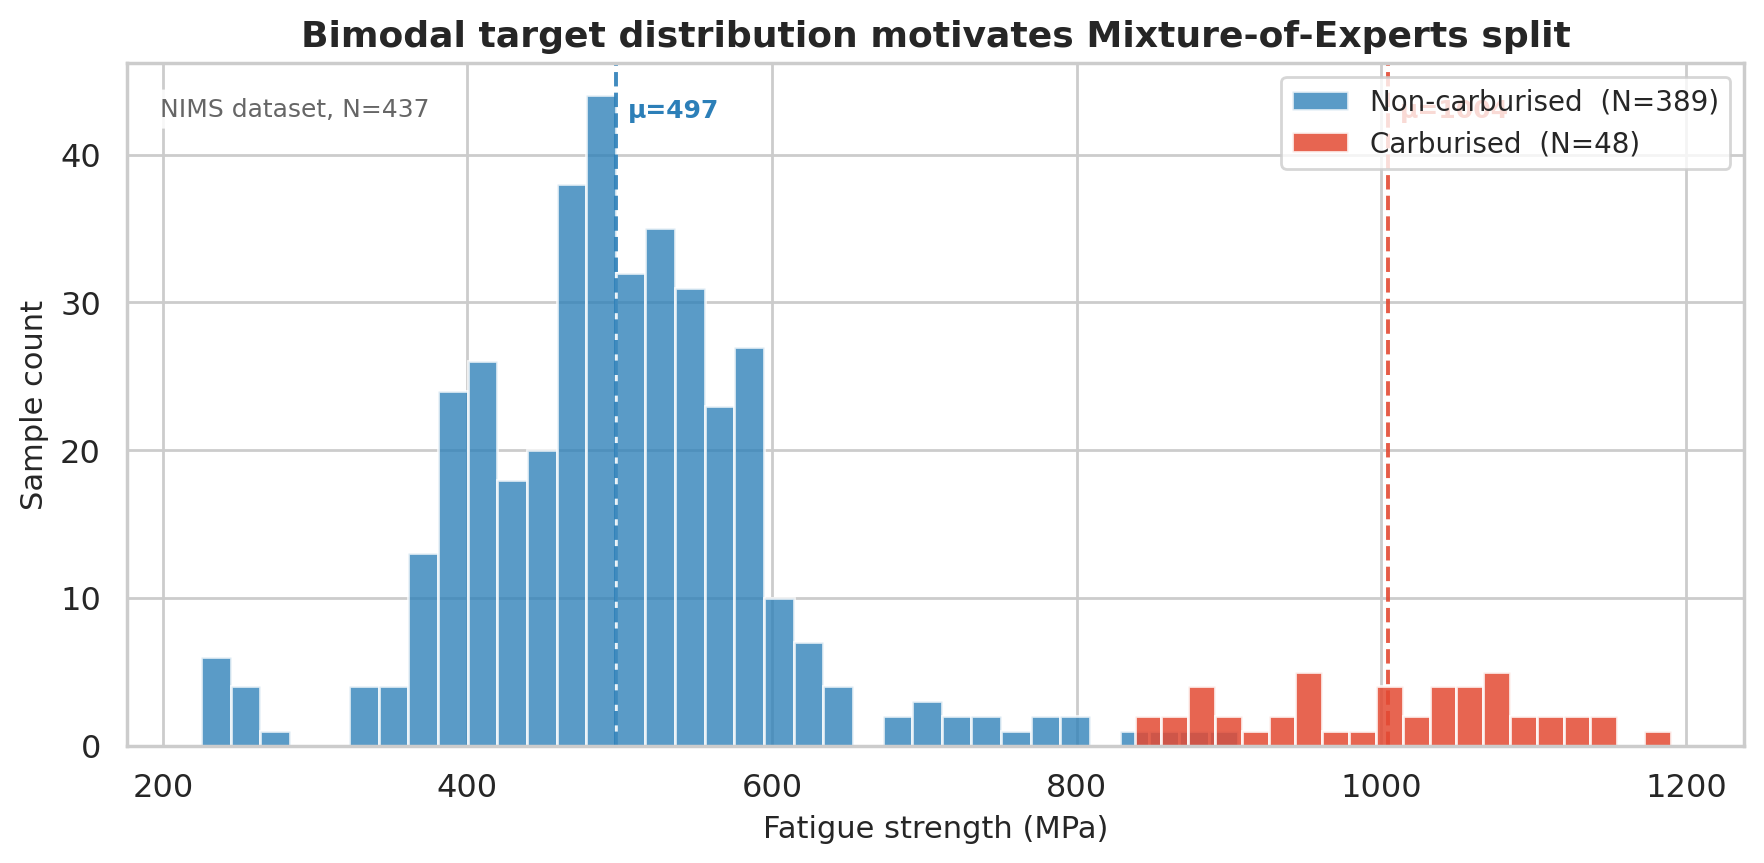
\includegraphics[width=0.62\textwidth]{slides_plots/01_bimodality.png}
\caption{NIMS fatigue distribution ($N=437$). Bimodal: NC ($\mu=497$\,MPa, blue) vs.\ carburised ($\mu\approx1007$\,MPa, red). Gap $>$250\,MPa motivates separate experts.}
\label{fig:bimodal}
\end{figure}

\subsection{Applicability Boundary}
The dataset is overwhelmingly populated by alloyed low-alloy steels with non-zero Cr,
Mn, and often Mo or Ni. External validation (§\ref{sec:ext}) shows that the learned
mapping does not transfer reliably to plain-carbon grades. We therefore explicitly
restrict the deployed model to the alloyed regime
\[
  \text{Cr} + \text{Ni} + \text{Mo} \ge 0.1~\text{wt\%},
\]
and treat violations of this threshold as out-of-scope rather than as a soft warning. That
boundary is not cosmetic: it follows directly from the training distribution and is
confirmed by both handbook checks and the OOD matbench probe.


% ─────────────────────────────────────────────────────────────────────────────
\section{Final Architecture}\label{sec:arch}
% ─────────────────────────────────────────────────────────────────────────────

\begin{figure}[H]
\centering
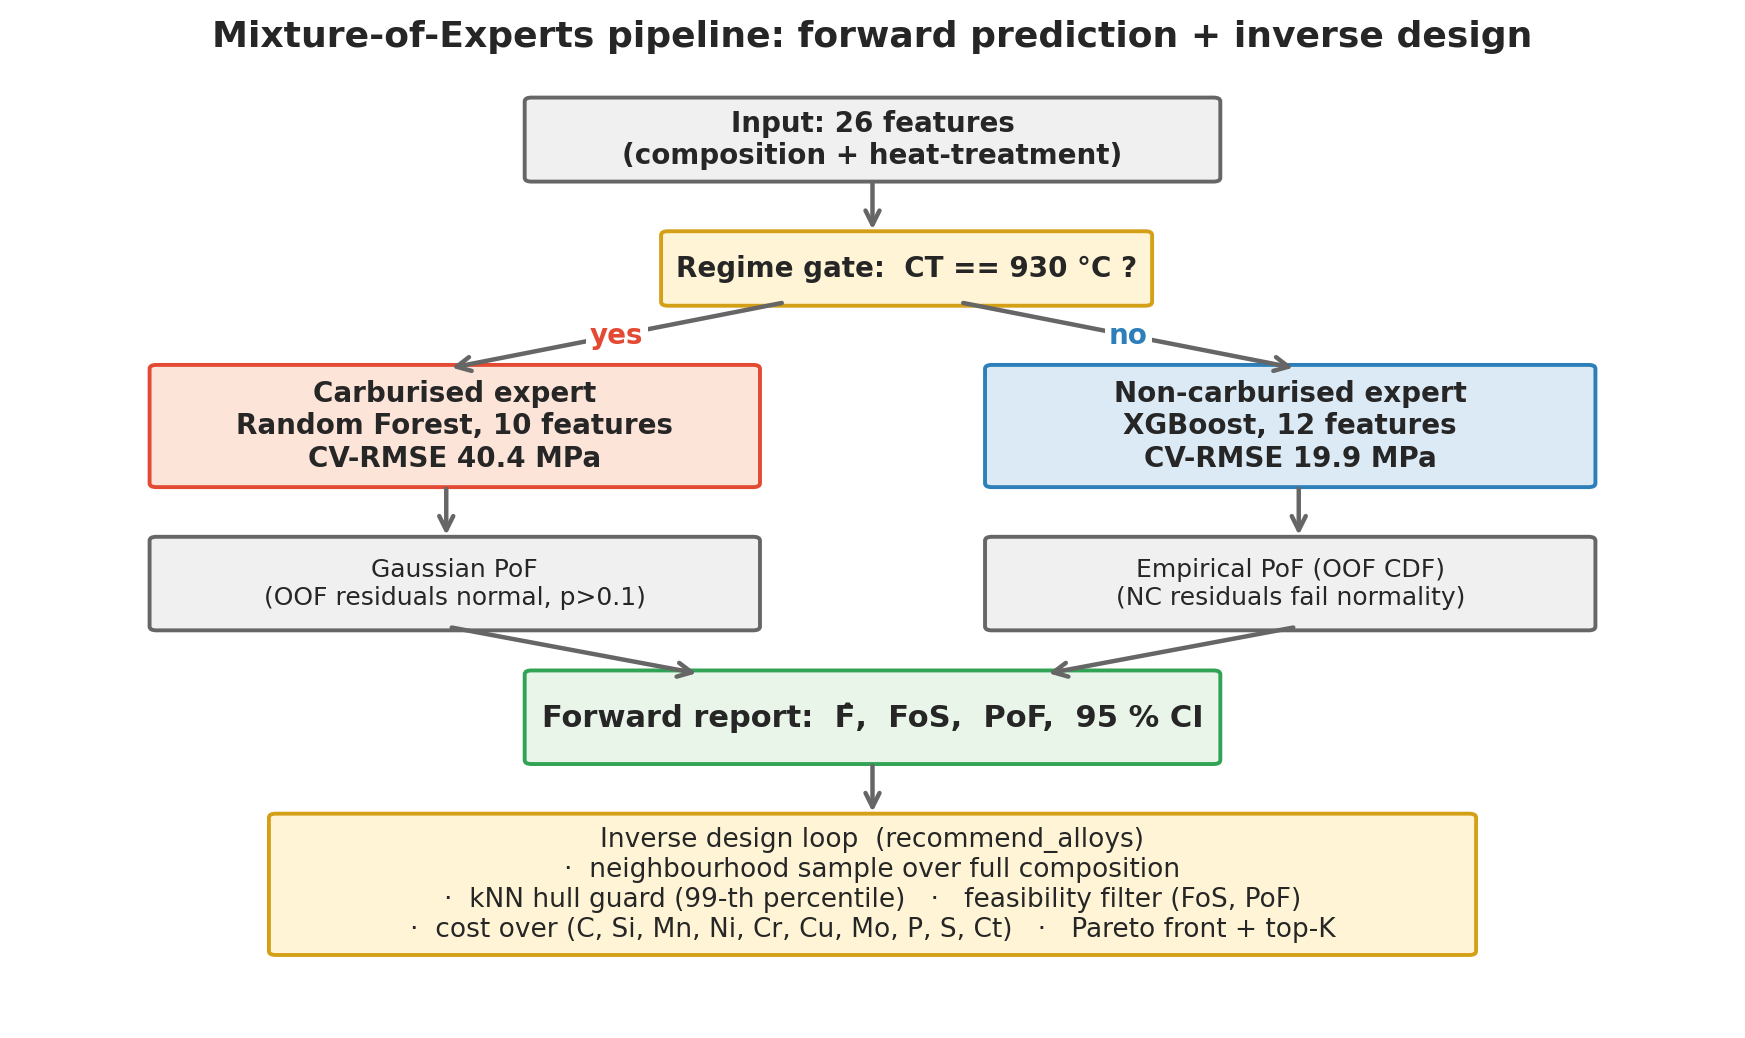
\includegraphics[width=0.78\textwidth]{slides_plots/02_architecture.png}
\caption{Pipeline. Gate ($CT=930\,^\circ$C) routes to NC expert (XGBoost, 16 feat, 19.2\,MPa) or C expert (RF, 7 feat, 40.1\,MPa). Both feed forward report and inverse design.}
\label{fig:arch}
\end{figure}

\subsection{Why Mixture-of-Experts (MoE)}\label{sec:moe}
A single global model averages two physically distinct strengthening mechanisms
(case-hardening vs.\ through-hardening) and produces an inflated, regime-blind error.
We engineer a binary gate
\[
  \texttt{is\_carburized} = \mathbf{1}[\,CT = 930\,]
\]
and route to two independent experts.

\textbf{Note.} A tuned global XGBoost lands in the same pooled-RMSE ballpark
($\sim$23\,MPa) as the MoE pair. The gain from the split is therefore not simply point
accuracy. It is calibration. The carburised and non-carburised populations exhibit
different target ranges, different residual shapes, and different physically meaningful
uncertainty scales. A single pooled model can obscure those differences even when its
overall RMSE looks competitive. The MoE architecture preserves them explicitly, which is
why it is the right foundation for calibrated Probability of Failure reporting.

\subsection{Per-regime Model Choice}
We benchmark four candidate model families on the regime-specific features under
5-fold cross-validation, using default hyperparameters to isolate the effect of model
class:

\begin{table}[H]
\centering
\caption{Untuned 5-fold CV RMSE per regime. Bold = chosen family.}
\label{tab:benchmark}
\begin{tabular}{lrr}
\toprule
\textbf{Model} & \textbf{NC RMSE (MPa)} & \textbf{C RMSE (MPa)} \\
\midrule
\textbf{XGBoost} & \textbf{24.22 ± 2.49} & 52.49 ± 17.57 \\
\textbf{Random Forest} & 25.96 ± 1.90 & \textbf{44.31 ± 11.89} \\
Ridge            & 28.85 ± 0.79 & 68.36 ± 16.32 \\
kNN ($k=7$)      & 72.02 ± 8.14 & 72.25 ± 7.07 \\
\bottomrule
\end{tabular}
\end{table}

\textbf{NC (XGBoost).} Tuned XGBoost reaches 19.2\,MPa, the lowest CV-RMSE in the
benchmark. In the larger non-carburised branch, boosting has enough data to exploit
non-linear interactions between chemistry and treatment variables without becoming
unstable. It also handles the right-skewed target effectively without an explicit response
transform.

\textbf{C (Random Forest).} With $N\,{=}\,48$, RF's bagging and aggressive depth-limit make
it strictly more robust than XGBoost's boosting cascade. In the carburised branch, the
central problem is variance control rather than expressivity. Bagging, depth limits, and
leaf regularisation therefore matter more than raw non-linear flexibility. Tuned RF:
40.1\,MPa.

\begin{figure}[H]
\centering
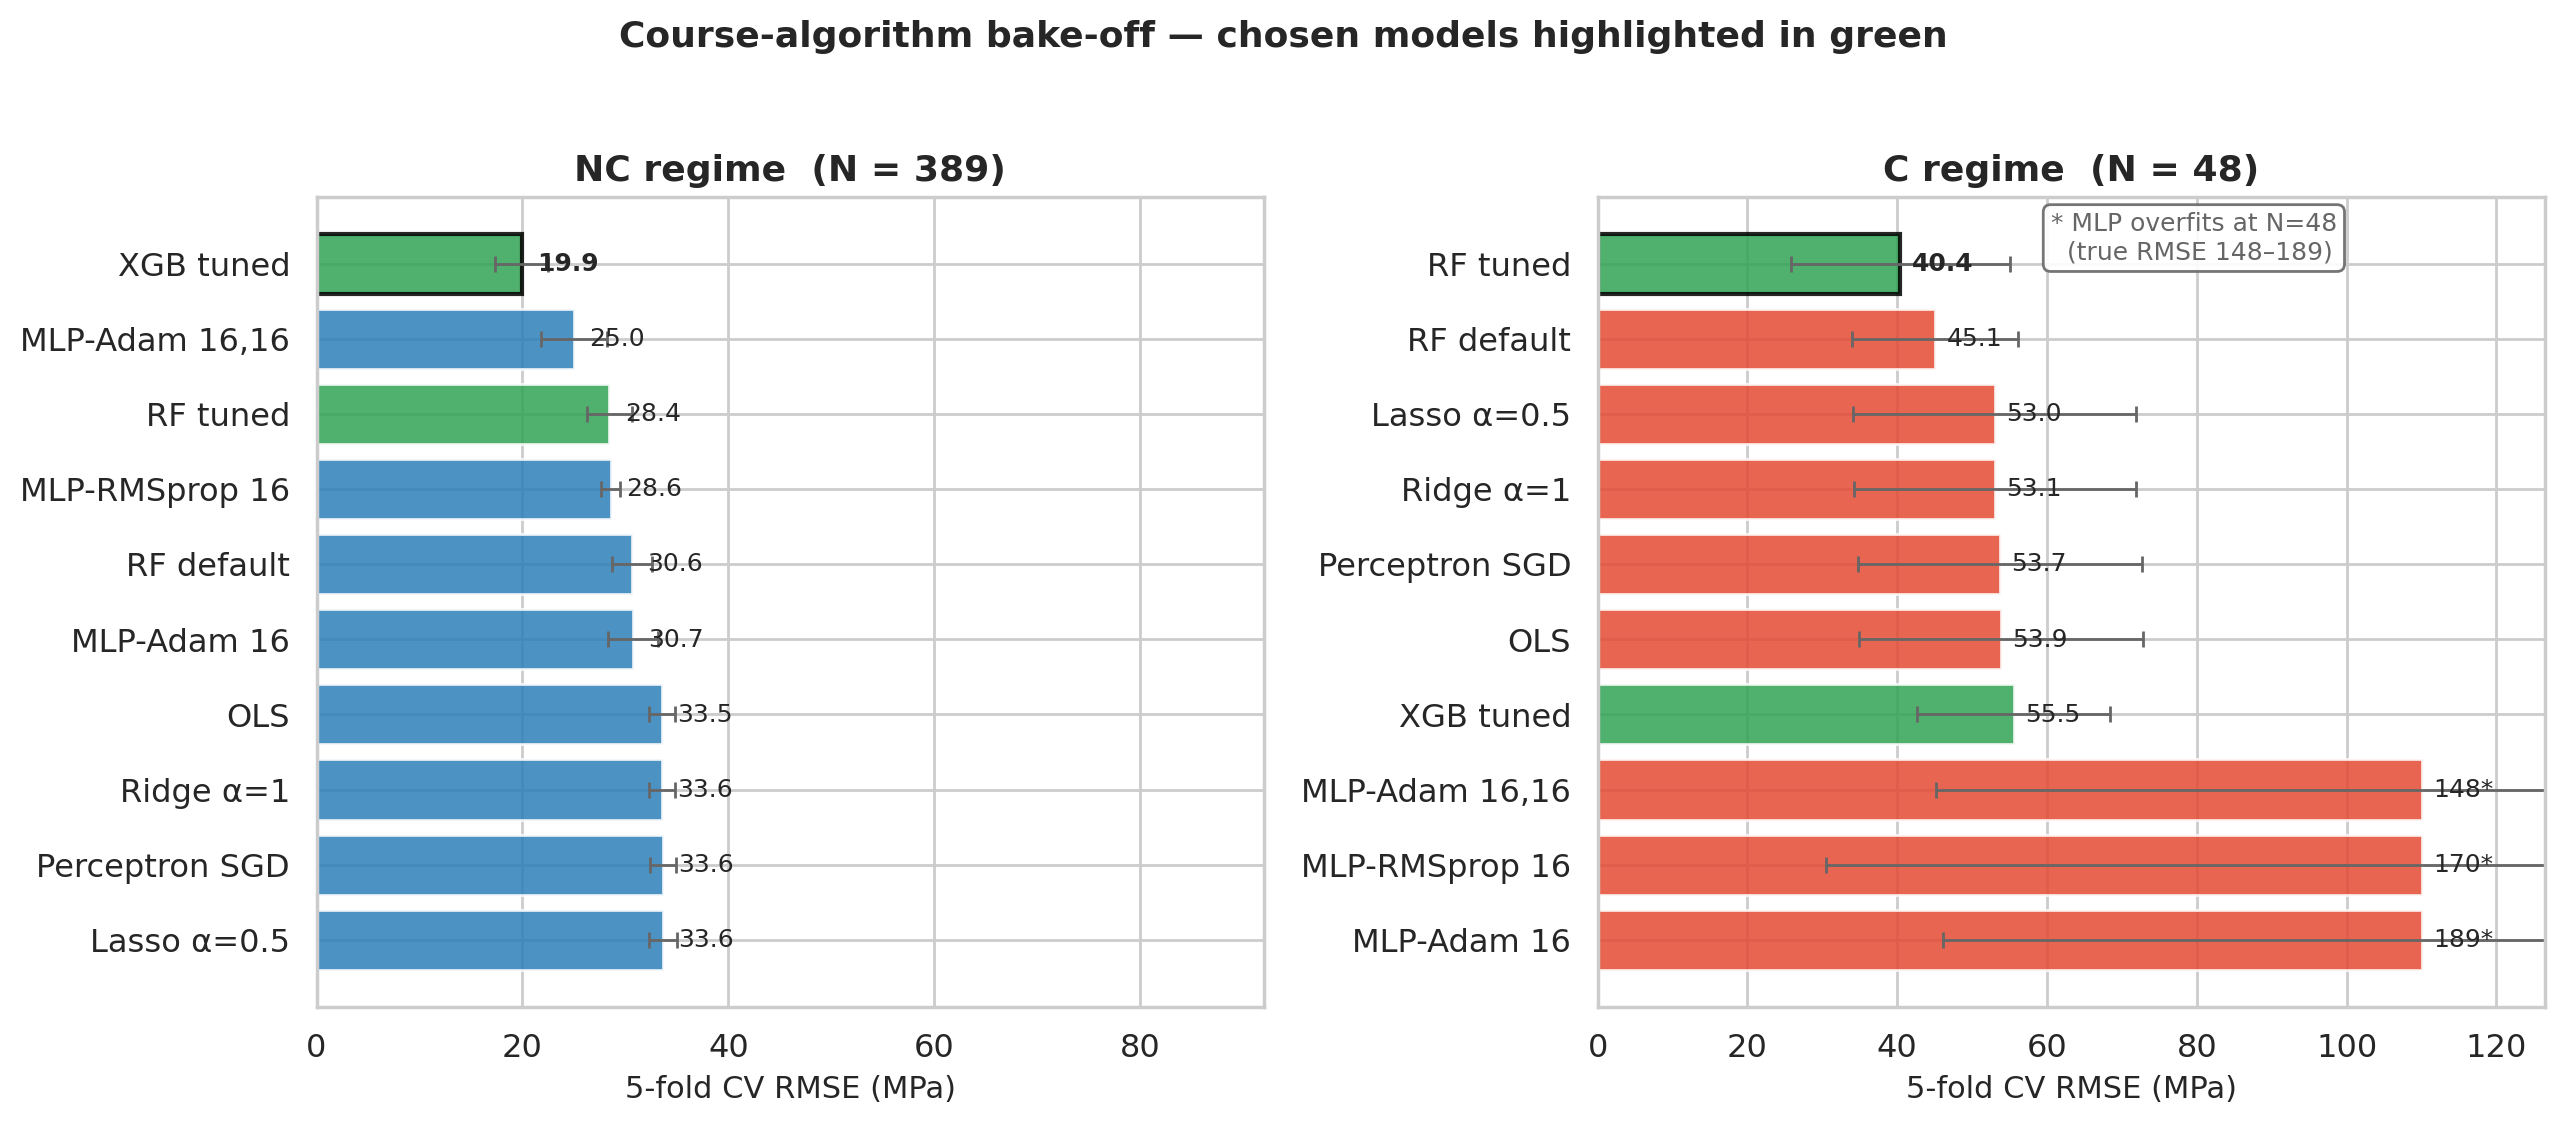
\includegraphics[width=0.70\textwidth]{slides_plots/03_bakeoff.png}
\caption{5-fold CV RMSE per regime (chosen models in green). NC: XGBoost 19.2\,MPa leads. C: RF 40.1\,MPa leads while MLP variants remain unstable at $N=48$.}
\label{fig:benchmark}
\end{figure}

\subsection{Feature Selection \texorpdfstring{(VIF $\rightarrow$ SHAP)}{(VIF to SHAP)}}
The 26 raw features contain heavy collinearity (e.g.\ CT, DT, QmT all encode the same
thermal cycle). We apply a two-stage reduction:
\begin{enumerate}[nosep]
  \item \textbf{VIF filter:} iteratively drop the feature with the largest variance
        inflation factor until all VIF\,$<$\,10. Drops 6 features per regime.
  \item \textbf{SHAP scout:} fit a shallow Random Forest on VIF survivors and retain the
        top-$k$ features by mean $|\,\text{SHAP}\,|$. Optuna tunes $k$ jointly with the
        downstream model; the deployed values are $k=16$ for NC and $k=7$ for C.
\end{enumerate}

\paragraph{No data leakage.} Both stages are encapsulated in
\texttt{VIFThenShapSelector}, a custom \texttt{scikit-learn} transformer, and composed
with the downstream estimator inside a single \texttt{Pipeline}. When that pipeline is
evaluated under \texttt{cross\_val\_score}, the VIF filter and the SHAP-scout Random
Forest are re-fitted on each training fold only; the held-out fold never participates in
feature selection. The reported CV-RMSE values ($19.19 \pm 2.52$\,MPa for NC and
$40.06 \pm 13.69$\,MPa for C) are therefore honest leakage-free generalisation
estimates. The final feature lists below are extracted from a single full-data fit after CV
has finished, and are used solely for deployment.

\begin{table}[H]
\centering
\caption{Final selected features per regime.}
\label{tab:features}
\begin{tabular}{ll}
\toprule
\textbf{Regime} & \textbf{Selected features} \\
\midrule
Non-carburised & Cr, TT, C, Mn, THT, Mo, Si, RedRatio, P, S, dA, Cu, Ni, dB, dC, QmT \\
Carburised     & P, RedRatio, Ct, Mo, S, Mn, Cu \\
\bottomrule
\end{tabular}
\end{table}

\paragraph{Physical interpretation.} For non-carburised steels, tempering temperature
(TT) and chromium remain dominant, consistent with martensite tempering and
hardenability theory, while Ni and the inclusion / quench descriptors (dB, dC, QmT)
survive because the larger NC sample size supports a slightly richer signal. For
carburised steels, the selected set is deliberately compact: carburising time (Ct),
reduction ratio (RedRatio), molybdenum, and manganese capture most of the useful
variation in case-hardening performance.

\subsection{Hyperparameter Tuning}
Optuna TPE search, up to 200 trials, with 5-fold CV as the objective.
Each Optuna trial jointly chooses the model hyperparameters and the number of SHAP
features to retain, then evaluates the entire selector-plus-model pipeline under 5-fold CV.
The objective value is the mean RMSE across the five held-out folds, so Optuna is tuning
against out-of-fold validation error rather than training error. This inner CV loop is used
only for model selection. Separately, an 80/20 stratified holdout split by fatigue quintile
is kept entirely outside Optuna as a final sanity check; once the holdout agrees with the
CV picture, the deployed experts and their final feature lists are obtained from a refit on
the full regime data using the selected recipe.
The search now uses a plateau-based early-stop rule: after at least 60 trials, the study is
halted once best CV RMSE fails to improve by 0.01\,MPa for 40 consecutive trials. In the
final deployed runs, this ended the NC and C searches after 124 and 145 trials
respectively, while still preserving the stronger minima.
This matters because the value of a hyperparameter setting depends on the feature subset it
ultimately sees, and conversely the best feature subset depends on the model family and its
regularisation. Joint tuning therefore avoids the common pitfall of optimising the model on
a feature space selected under a different criterion.

\begin{table}[H]
\centering
\caption{Best hyperparameters from Optuna.}
\label{tab:hparams}
\begin{tabular}{lll}
\toprule
\textbf{Parameter} & \textbf{NC XGBoost} & \textbf{C Random Forest} \\
\midrule
n\_estimators       & 311                 & 238 \\
max\_depth          & 4                   & 4 \\
learning\_rate      & 0.064               & --- \\
subsample           & 0.934               & --- \\
colsample\_bytree   & 0.735               & --- \\
min\_child\_weight  & 2                   & --- \\
reg\_alpha          & 0.0003              & --- \\
reg\_lambda         & 0.483               & --- \\
min\_samples\_split & ---                 & 9 \\
min\_samples\_leaf  & ---                 & 4 \\
max\_features       & ---                 & 0.797 \\
\bottomrule
\end{tabular}
\end{table}


% ─────────────────────────────────────────────────────────────────────────────
\section{Reliability: Empirical PoF}\label{sec:reliability}
% ─────────────────────────────────────────────────────────────────────────────

The deployment wrapper maps a prediction to a Probability of Failure under applied stress
$\sigma_{\text{app}}$:
\[
  \text{PoF} = P(F < \sigma_{\text{app}})
\]
where $F$ is the realised fatigue strength of a fresh specimen.
That quantity is the central safety-facing output of the system. A point prediction alone
is insufficient for engineering use because design decisions depend on where the applied
stress sits relative to predictive uncertainty. Our reliability layer therefore asks a
distributional question: given the model and its observed residual behaviour, what is the
probability that a fresh specimen falls below the requested load?

\subsection{Limitations of the Gaussian Assumption}
A first-pass approach uses
$\text{PoF} = \Phi\!\big((\sigma_{\text{app}} - \hat{F}) / \sigma_{\text{CV}}\big)$.
This is correct only when the residuals $r = F - \hat{F}$ are Gaussian.

\textbf{Test on OOF residuals}: training-fit residuals are optimistically biased and
artificially narrow because they reflect in-sample interpolation. To validate the Gaussian
assumption honestly, we must inspect out-of-fold (OOF) residuals generated under the same
5-fold structure as the reported CV RMSE.

\begin{table}[H]
\centering
\caption{Residual normality on OOF predictions vs.\ training fit.}
\label{tab:residuals}
\setlength{\tabcolsep}{5pt}
\begin{tabular}{l l r p{3.4cm} r r}
\toprule
\textbf{Regime} & \textbf{Source} & \textbf{Std (MPa)}
                & \textbf{Range (MPa)} & \textbf{Shapiro $p$} & \textbf{KS $p$} \\
\midrule

NC & Train fit            &  5.54 & $-34.3$ to $+27.3$    & 0.0000 & 0.4236 \\
NC & \textbf{OOF}         & \textbf{20.12} & \textbf{$-97.5$ to $+108.3$}
                                                           & \textbf{0.0000} & \textbf{0.0002} \\
C  & Train fit            & 34.29 & $-96.3$ to $+81.4$    & 0.2283 & 0.3787 \\
C  & \textbf{OOF}         & \textbf{42.39} & \textbf{$-112.2$ to $+93.4$}
                                                           & 0.3788 & 0.5684 \\
\bottomrule
\end{tabular}
\end{table}

\textbf{Conclusion.}
\begin{itemize}[nosep]
  \item NC OOF residuals fail \emph{both} normality tests ($p < 0.001$) — heavy right tail.
        Gaussian PoF is invalid; we use the empirical CDF.
  \item C OOF residuals pass both tests; Gaussian PoF is valid.
\end{itemize}

\begin{figure}[H]
\centering
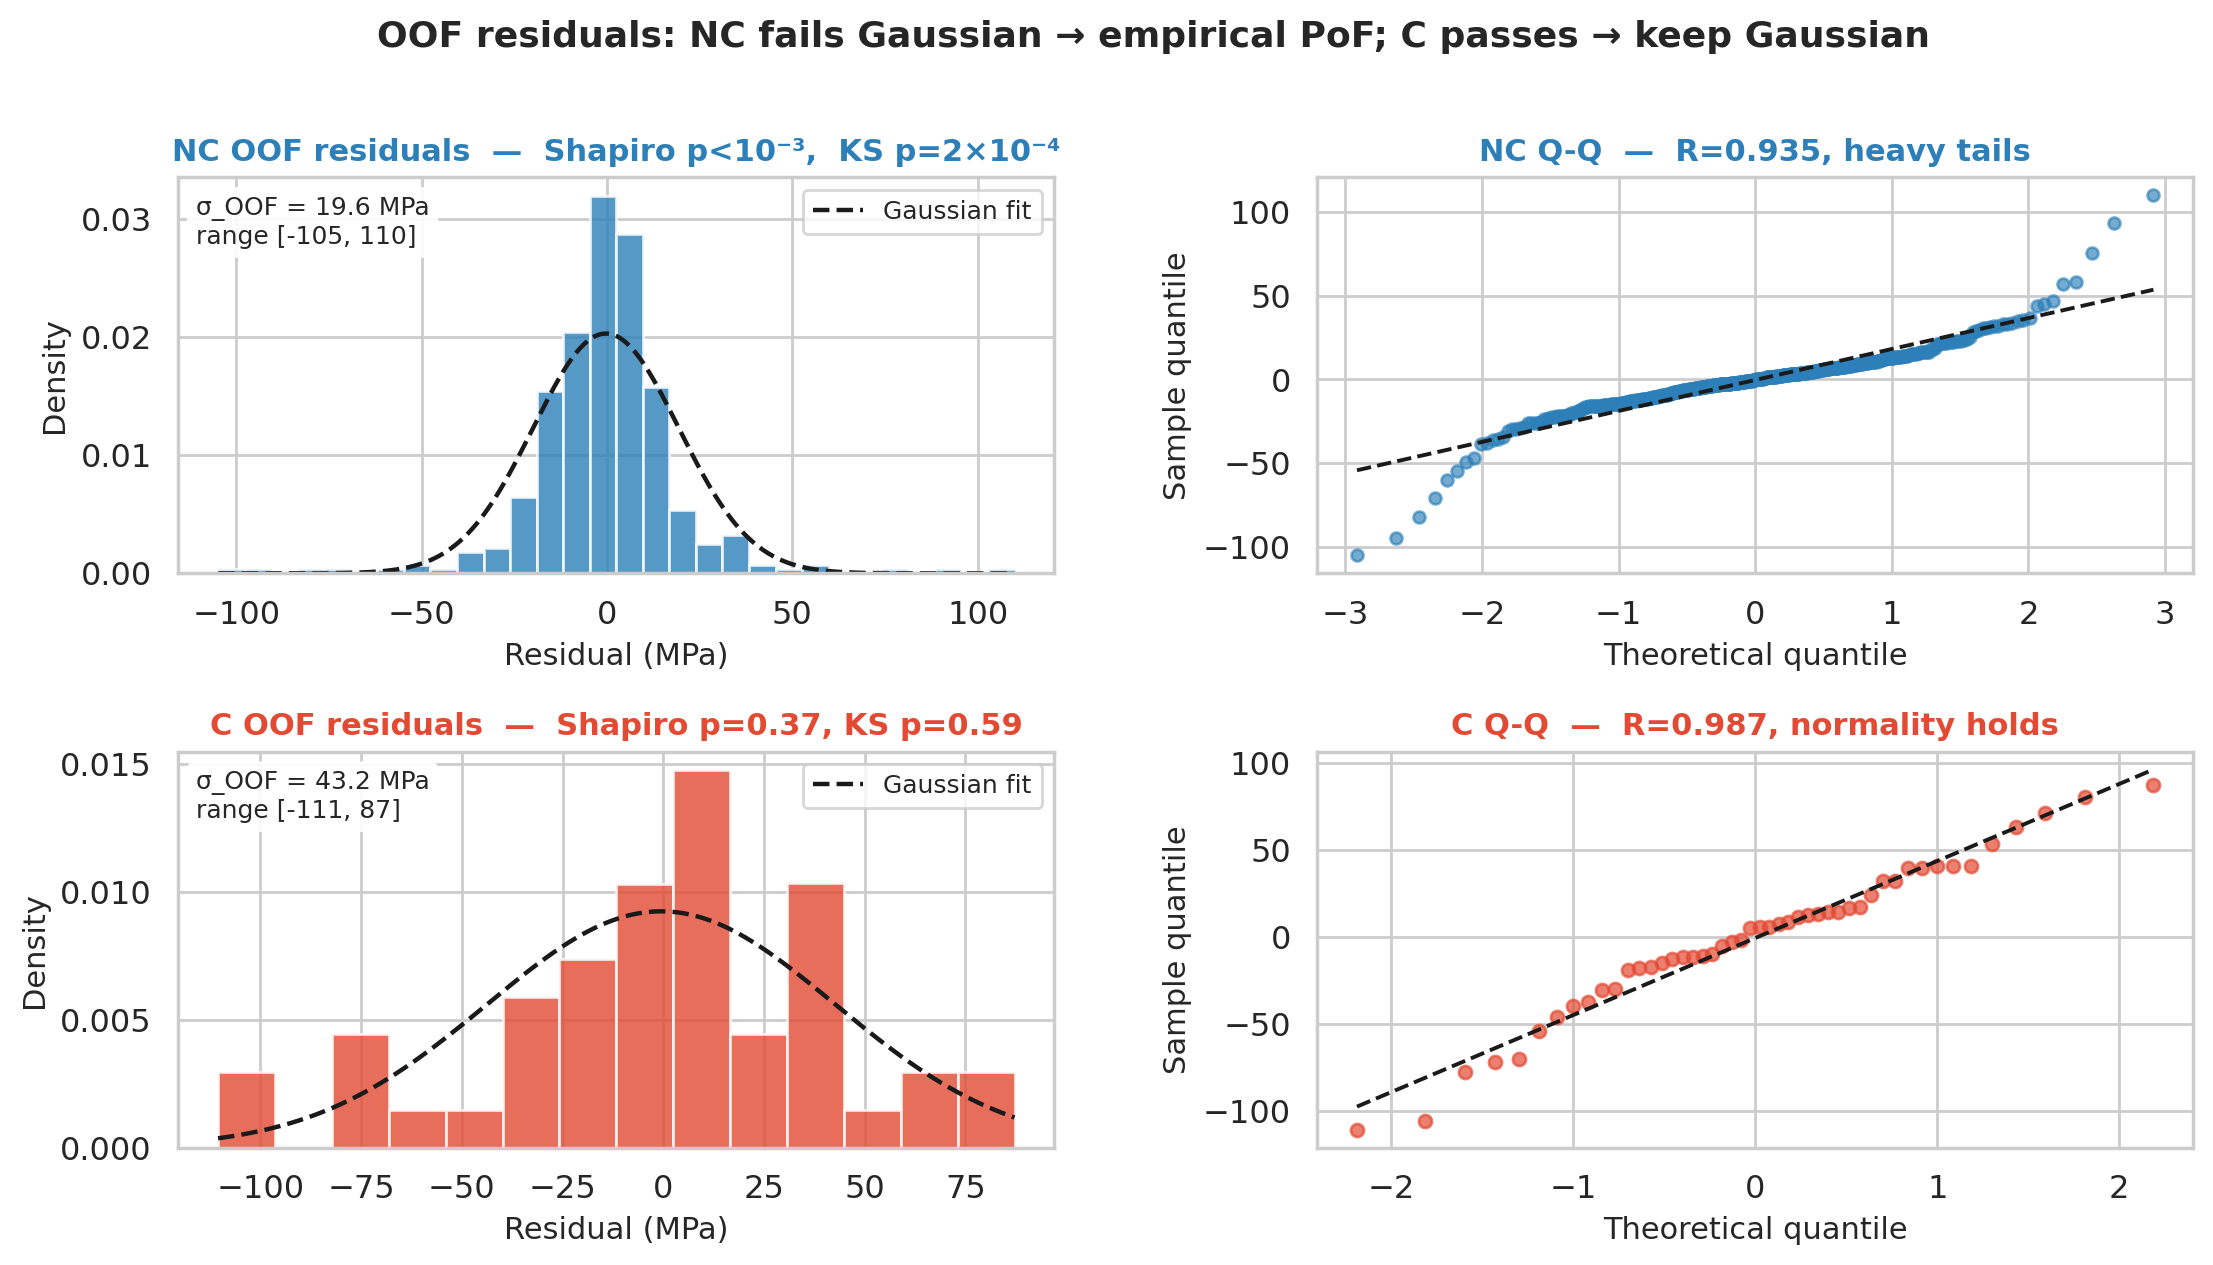
\includegraphics[width=0.68\textwidth]{slides_plots/04_oof_residuals.png}
\caption{OOF residual diagnostics. NC (top): heavy tails, Shapiro $p<10^{-3}$ --- empirical CDF required. C (bottom): normal ($p=0.38$) --- Gaussian PoF valid.}
\label{fig:oof}
\end{figure}

\subsection{Empirical PoF Formula (NC)}
We pre-compute OOF residuals $\{r_i\}_{i=1}^{389}$ at startup. For a candidate with
predicted fatigue $\hat{F}$ at applied stress $\sigma_{\text{app}}$:
\[
  \text{PoF}_{\text{empirical}}
    = P(\hat{F} + r < \sigma_{\text{app}})
    = \frac{1}{389}\sum_{i=1}^{389}\mathbf{1}\!\left[r_i < \sigma_{\text{app}} - \hat{F}\right].
\]
This is the empirical CDF of residuals evaluated at the gap. It captures heavy tails and
asymmetry that $\Phi$ misses.

\paragraph{Magnitude of the correction.}
At $\sigma_{\text{app}} = 590$\,MPa, $\hat{F} = 585.0$\,MPa:
$\text{PoF}_{\text{Gaussian}} = 0.603$ vs.\ $\text{PoF}_{\text{empirical}} = 0.663$ --- 6.0\,pp difference. Gaussian is over-confident in the upper tail; at low applied stresses the discrepancy reverses and collapses at large margins.
This divergence is not a cosmetic calibration issue. Near the fatigue limit, a 6.0
percentage-point shift in failure probability is large enough to alter engineering
decisions about acceptable operating stress or the need for a more expensive alloy. At
lower applied stresses the Gaussian model becomes conservative instead, but the key point
is the same: the residual shape matters, and the NC branch cannot be safely reduced to a
single normal $\sigma$.

\begin{figure}[H]
\centering
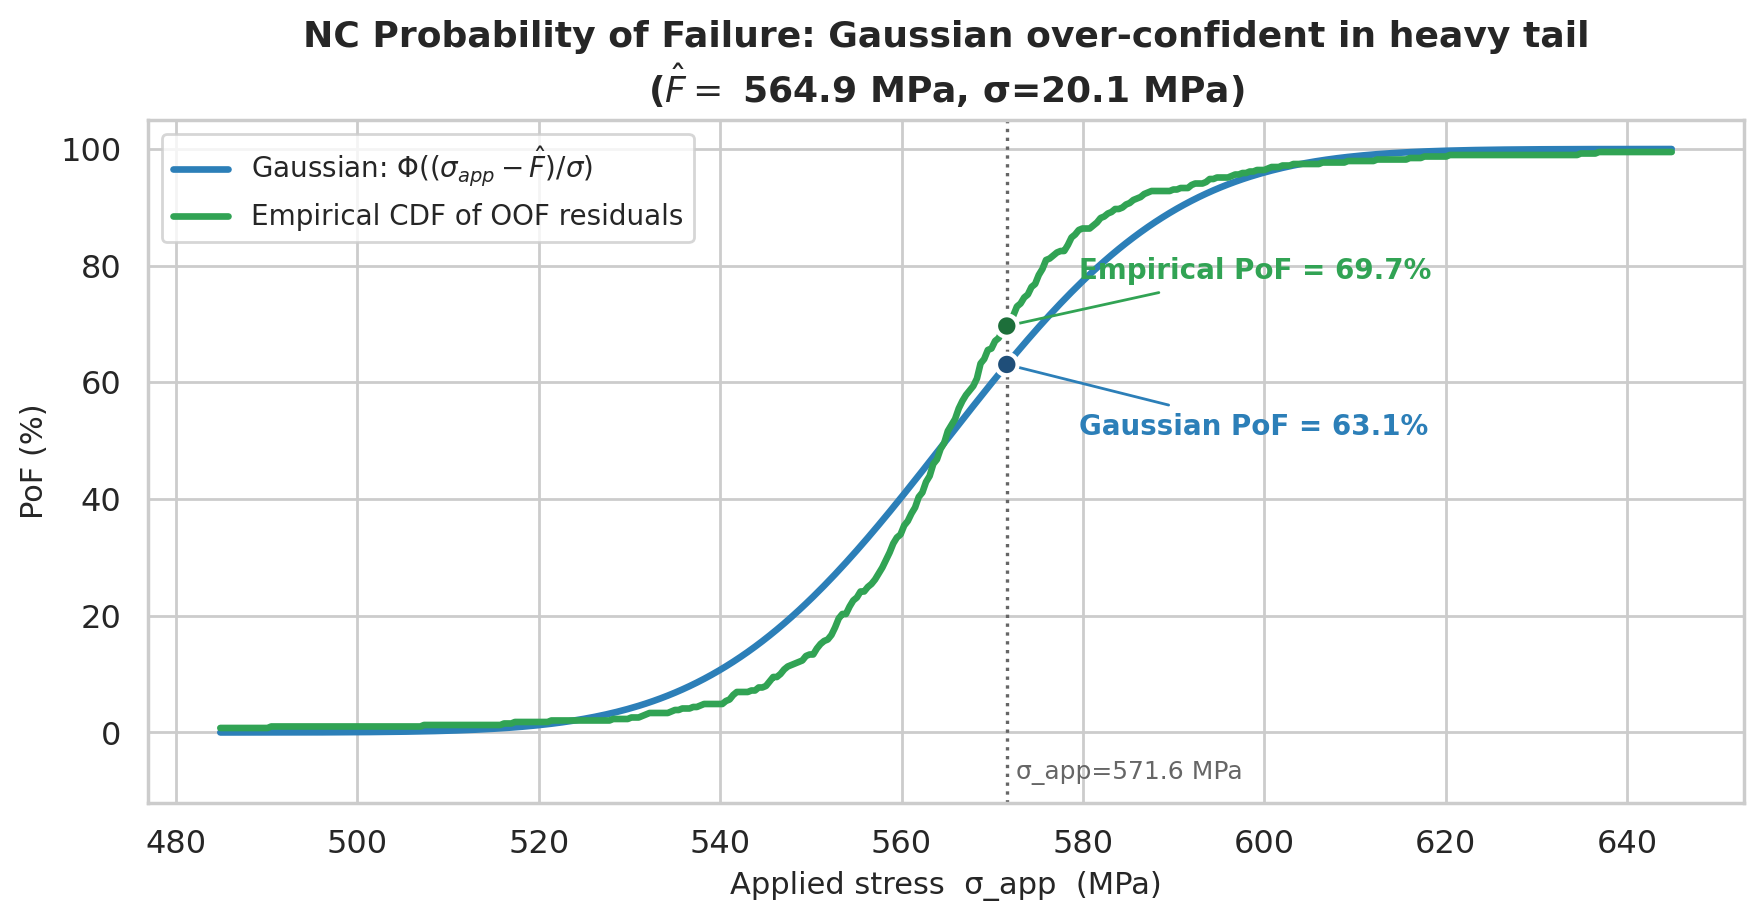
\includegraphics[width=0.58\textwidth]{slides_plots/05_pof_compare.png}
\caption{NC PoF curves ($\hat{F}=585.0$\,MPa). At $\sigma_{\text{app}}=590$\,MPa: Gaussian 60.3\,\% vs.\ empirical 66.3\,\% (+6.0\,pp). Gap vanishes at large safety margins.}
\label{fig:pof}
\end{figure}


% ─────────────────────────────────────────────────────────────────────────────
\section{Inverse Design}
% ─────────────────────────────────────────────────────────────────────────────

Given $\sigma_{\text{app}}$, target Factor of Safety FoS$^*$, and PoF cap $\tau$, find the
cheapest alloy $\mathbf{x}^*$ that satisfies:
\begin{align}
  \hat{F}(\mathbf{x}^*) &\geq \text{FoS}^* \cdot \sigma_{\text{app}}, \label{eq:fos}\\
  \text{PoF}(\mathbf{x}^*, \sigma_{\text{app}}) &\leq \tau, \label{eq:pof}\\
  \mathbf{x}^* &\in \mathcal{H}_{\text{train}}. \label{eq:hull}
\end{align}

\subsection{Neighbourhood Sampling (Full Composition)}
Latin Hypercube Sampling (LHS) over the bounding box wastes $>$\,99\,\% of samples on metallurgically impossible
combinations. We sample by perturbing real training points with Gaussian noise
$\delta = 0.20\,\hat{\sigma}_f$ per feature, clipped to per-feature bounds.
This choice is practical as much as statistical. The training set already encodes which
combinations of chemistry and process variables occur in physically plausible steels. By
sampling in the neighbourhood of known points, the inverse-design loop spends most of its
budget exploring meaningful local variations instead of generating random combinations
that are immediately rejected by the hull guard.

\textbf{Composition Union for Cost Modeling.}
The sampler unions predictive features with all cost-relevant elements \{C, Si, Mn, Ni, Cr, Cu, Mo, P, S, Ct\} to prevent falsely cheap rankings from omitted expensive elements (§\ref{sec:cost}).


\subsection{kNN Data-Hull Guard}
Constraint~\eqref{eq:hull} is enforced by a $k$-NN ($k=5$) filter. We standardise the
training features, fit kNN, and reject any candidate whose mean 5-NN distance exceeds the
99\textsuperscript{th} percentile of training-point self-distances.
The intent is not to guarantee strict physical feasibility in a first-principles sense, but
to prevent the inverse-design search from wandering into regions where the model is
performing unconstrained extrapolation. In practice this acts as a simple and auditable
data-support prior: if a candidate lies much farther from the observed training manifold
than any real training point lies from its neighbours, we do not trust the recommendation.

\paragraph{Sensitivity.} The threshold matters for the non-carburised regime:
tightening from p99 to p95 sharply shrinks the feasible set and raises the top-1 cost,
while the carburised regime is much more stable. We therefore report results at p99 and
warn that NC recommendations live near the data hull boundary.

\subsection{Cost Model}\label{sec:cost}
\begin{equation}
  C(\mathbf{x}) = \sum_{e\,\in\,\text{elements}} p_e\,w_e(\mathbf{x})
              + c_{\text{proc}}\,t_{Ct}, \quad c_{\text{proc}} = 0.05\,\text{USD/min}.
\end{equation}
Element prices $p_e$ (USD/kg, approximate LME spot): Mo 30, Ni 14, Cr 10, Cu 9, Mn 1.8,
Si 1.2, C 0.5; P, S impurities priced at 0.

\subsection{Pareto Front and Seed Stability}
The recommender returns:
\begin{enumerate}[nosep]
  \item All feasible alloys (FoS \& PoF satisfied).
  \item The Pareto front in (cost, PoF) space.
  \item The top-$K$ cheapest feasible alloys.
\end{enumerate}

\textbf{Algorithm Stability.} Across random seeds, the exact recipe can move even when the
best cost stays in the same band. This is a natural consequence of a flat optimum:
multiple nearby chemistries can satisfy the same FoS and PoF constraints at nearly the
same cost. We therefore present the output as a band of viable candidates rather than a
single brittle prescription.

\subsection{Final Recommendations}

\paragraph{NC} Target: $\sigma_{\text{app}}=500$\,MPa, FoS\,$\geq 1.5$, PoF\,$\leq 2$\,\%.
Top candidate (\$4.62/kg): $\hat{F}=788.1$\,MPa (FoS 1.58, PoF 0.0\,\%). Strategy: lean-alloy chemistry with Cr 0.17\,wt\%, C 0.55\,wt\%, Mn 0.75\,wt\%, and very low Ni/Mo, paired with THT 848\,°C and TT 489\,°C.
The important engineering takeaway is that the NC solution does not rely on heavily
alloyed chemistry. Instead, it exploits a balanced heat-treatment route and moderate
carbon / manganese levels to achieve the target cheaply while still preserving margin.

\paragraph{C} Target: $\sigma_{\text{app}}=700$\,MPa, FoS\,$\geq 1.4$, PoF\,$\leq 2$\,\%.
Top candidate (\$18.43/kg): $\hat{F}=1016.4$\,MPa (FoS 1.45, PoF 0.0\,\%). Strategy: 90\,min carburisation with modest Mo (0.13\,wt\%), Mn 0.68\,wt\%, and a chromium-rich supporting chemistry.
For the carburised branch, the model converges to a more expensive but metallurgically
familiar recipe: stronger alloying support, sustained carburisation time, and a chemistry
that resembles the real-world logic of grades such as 4320/8620.

\begin{figure}[H]
  \centering
  \begin{subfigure}[b]{0.48\textwidth}
    \centering
    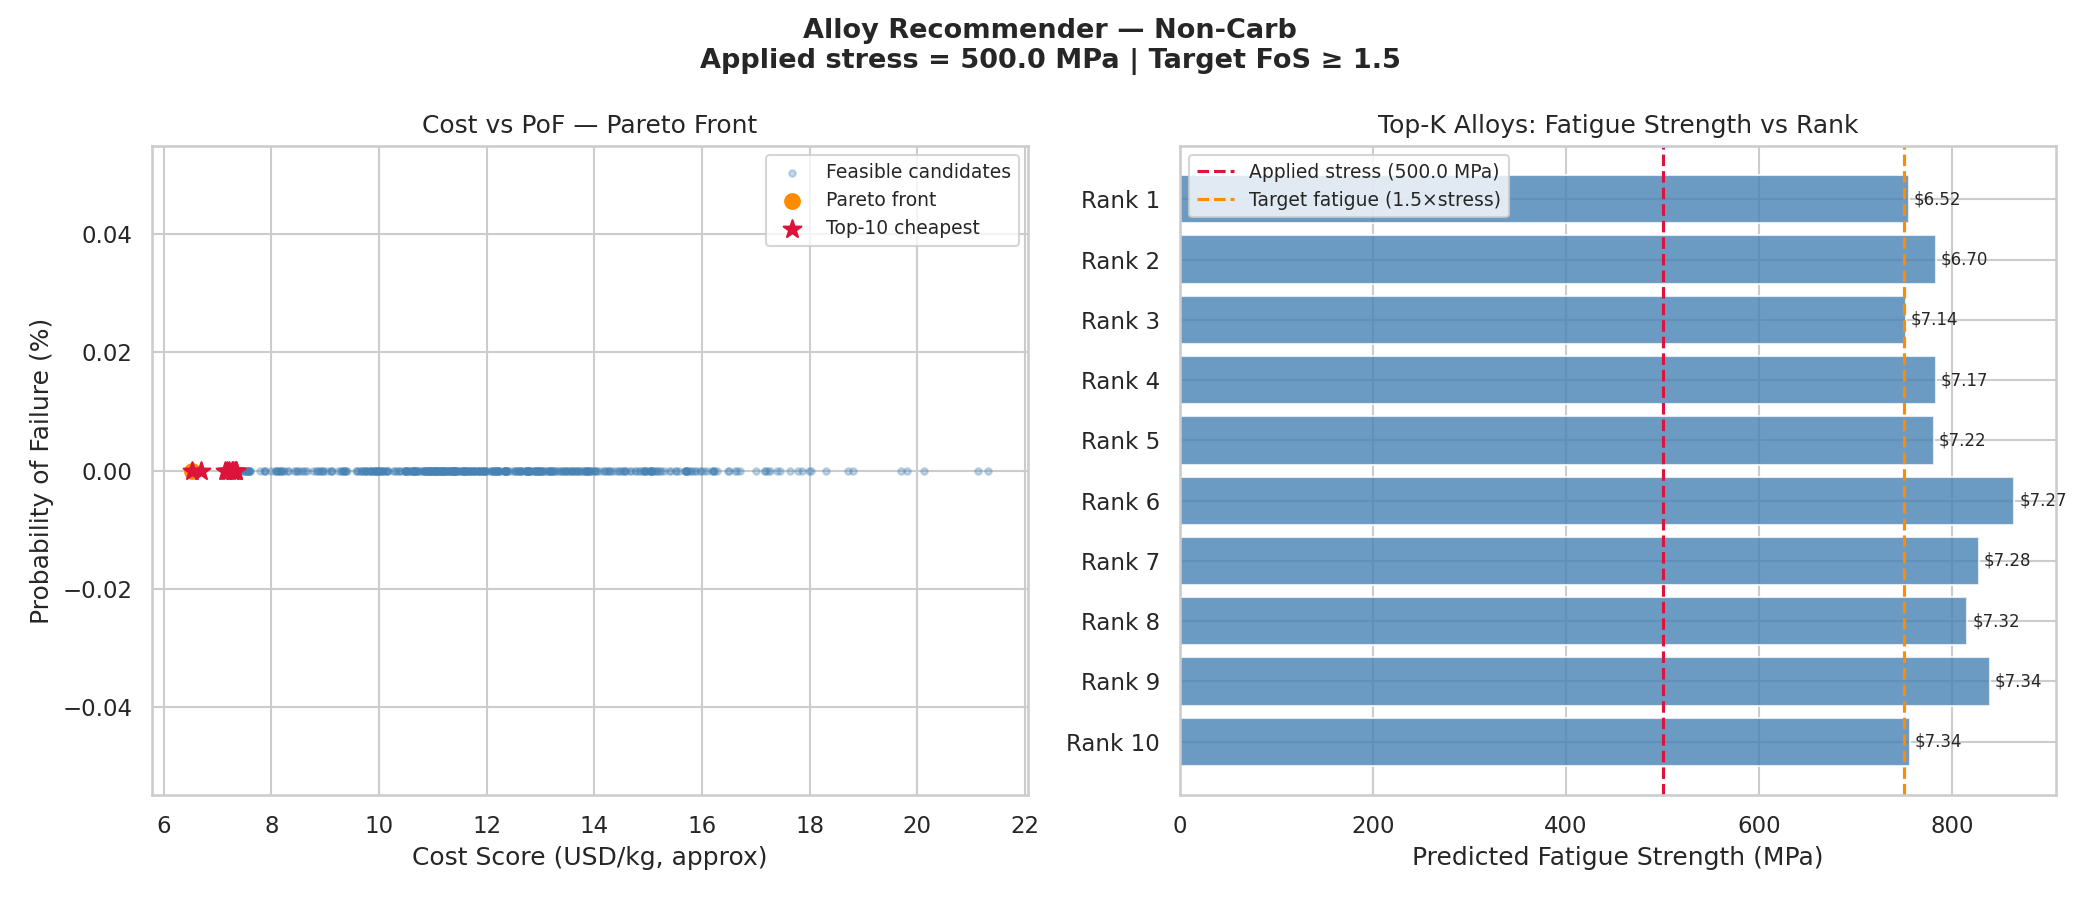
\includegraphics[width=\textwidth]{models/pareto_non_carb.png}
    \caption{Non-carburised.}
  \end{subfigure}
  \hfill
  \begin{subfigure}[b]{0.48\textwidth}
    \centering
    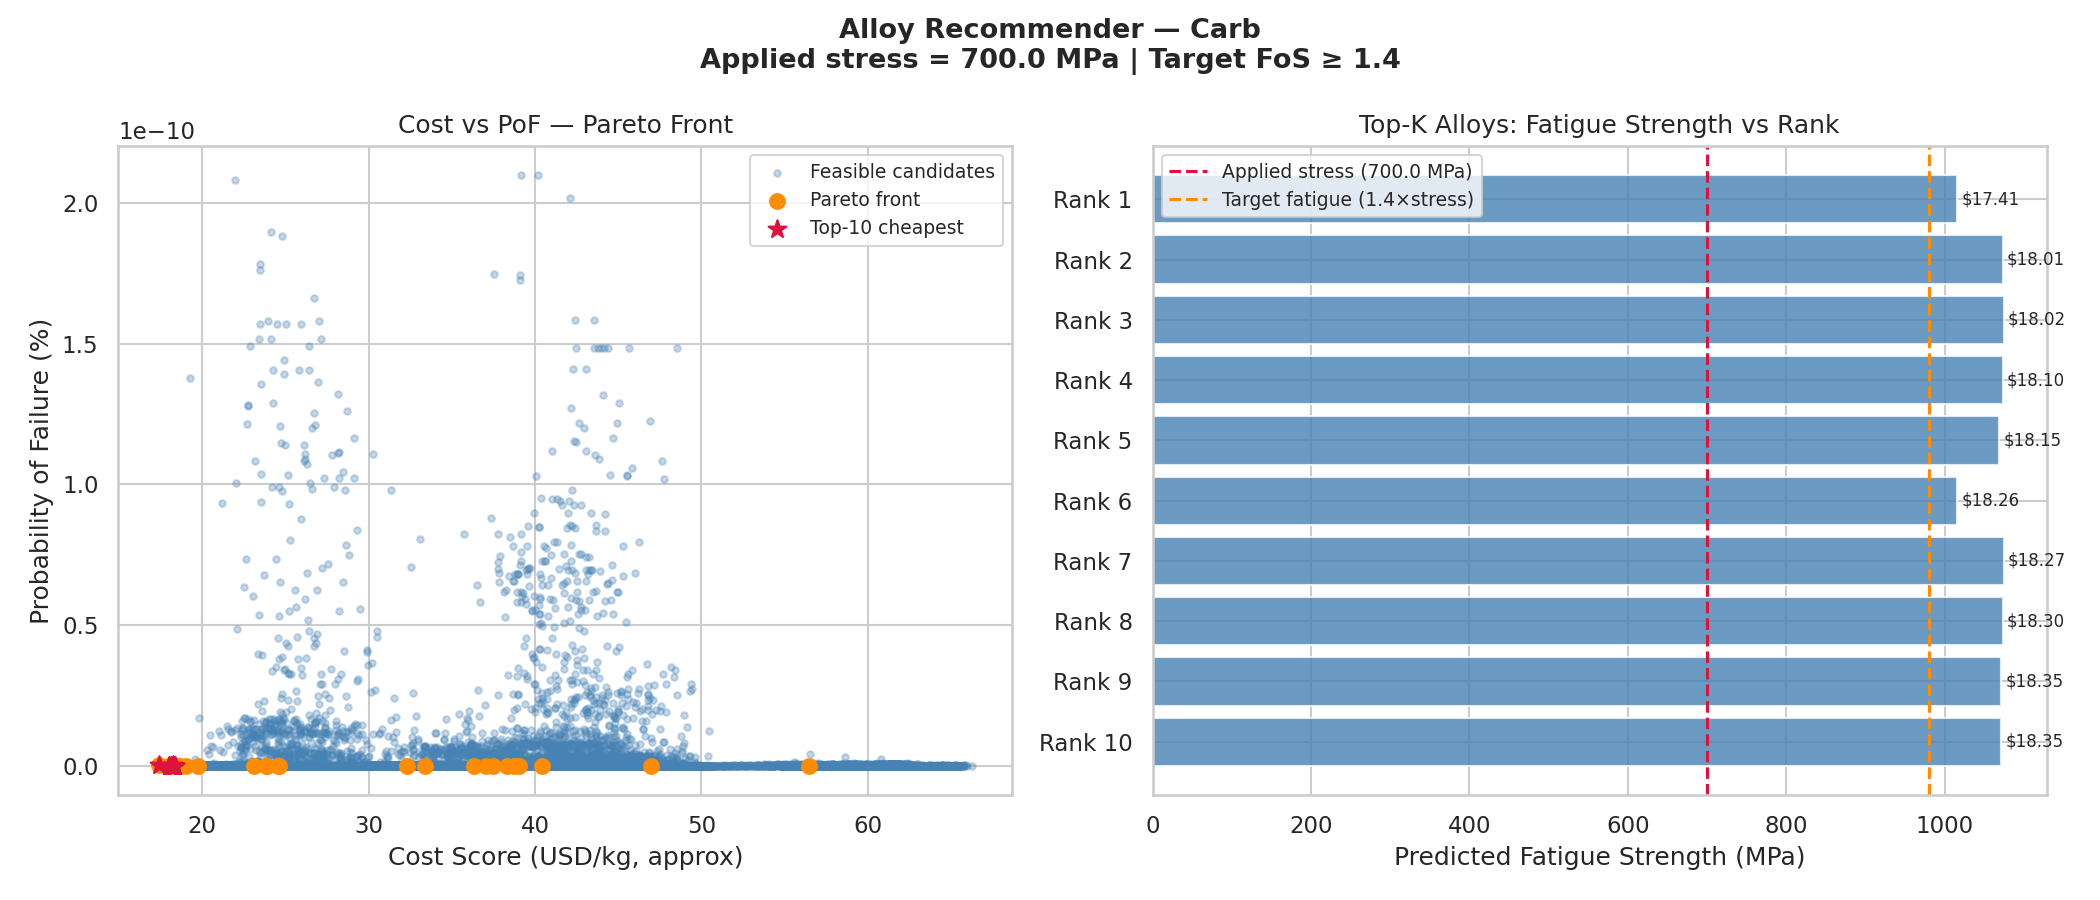
\includegraphics[width=\textwidth]{models/pareto_carb.png}
    \caption{Carburised.}
  \end{subfigure}
  \caption{Pareto front (cost vs.\ PoF). Orange: Pareto-optimal. Red stars: top-$K$ cheapest feasible alloys.}
  \label{fig:pareto}
\end{figure}

% ─────────────────────────────────────────────────────────────────────────────
\section{External Validation}\label{sec:ext}
% ─────────────────────────────────────────────────────────────────────────────

To determine not only whether the model predicts well, but also where it should and
should not be trusted, we validate it along three independent axes:

\subsection{Stratified NIMS Holdout (In-Distribution)}
80/20 stratified split by fatigue quintile (\texttt{random\_state=42}), held outside the
Optuna tuning loop.

\begin{table}[H]
\centering
\caption{Held-out test performance vs.\ 5-fold CV.}
\label{tab:holdout}
\begin{tabular}{lrrrr}
\toprule
\textbf{Regime} & \textbf{$N_{\text{train}}$ / $N_{\text{test}}$} & \textbf{Holdout RMSE} & \textbf{$R^2$} & \textbf{CV RMSE} \\
\midrule
NC & 311 / 78 & 17.93\,MPa & 0.973 & 19.19\,MPa \\
C  & 38 / 10  & 25.14\,MPa & 0.892 & 40.06\,MPa \\
\bottomrule
\end{tabular}
\end{table}

\textbf{Takeaway:} Holdout RMSE is at or below CV estimates, which is exactly what we
would hope to see from a well-disciplined CV pipeline. There is no sign that the models
are merely exploiting fold structure or benefiting from accidental leakage.

\subsection{Cross-Dataset Boundary Probe (\texttt{matbench\_steels})}
We applied the NC model (composition-only) to \texttt{matbench\_steels} (312 maraging alloys, yield-strength labels). Result: Spearman $\rho=-0.04$ ($p=0.44$) — no rank transfer; Pearson $r=-0.35$ ($p<0.001$). This confirms the applicability boundary: the model safely fails on out-of-distribution Co/Ni/V/W/Ti-rich maraging grades.
This is a useful negative result. The model was never intended to extrapolate into
maraging or ultra-high-strength chemistries, and the absence of rank transfer confirms that
it does not spuriously appear accurate outside its training family.

\subsection{Canonical Handbook Grades}
We supplied mid-range handbook compositions~\cite{shigley} for four AISI grades and checked predictions against published rotating-bending fatigue ranges.

\begin{table}[H]
\centering
\caption{Predictions on canonical AISI grades. Handbook ranges from Shigley / ASM.}
\label{tab:grades}
\begin{tabular}{lrcrrl}
\toprule
\textbf{Grade} & \textbf{Pred (MPa)} & \textbf{Regime} & \textbf{HB lo} & \textbf{HB hi} & \textbf{Status} \\
\midrule
AISI 1045 (norm.)    & 501.9 & NC & 260 & 340  & \textbf{HIGH (+162)} \\
AISI 4140 QT         & 654.8 & NC & 450 & 620  & \textbf{HIGH (+35)}  \\
AISI 4340 QT         & 662.1 & NC & 520 & 660  & \textbf{HIGH (+2)}   \\
AISI 8620 carb.      & 923.8 & C  & 700 & 1000 & OK                   \\
\bottomrule
\end{tabular}
\end{table}

\textbf{Takeaway:} 1/4 grades fall strictly within handbook ranges. AISI 8620 remains
in-range, 4340 QT is nearly exact (+2\,MPa), 4140 QT stays slightly high (+35\,MPa), and
AISI 1045 (Cr\,$<$\,0.1\,wt\%) remains strongly over-predicted (+162\,MPa), confirming the
plain-carbon boundary. The deployed GUI therefore enforces
Cr+Ni+Mo\,$\geq$\,0.1\,wt\% rather than pretending to generalise to unalloyed steels.

\begin{figure}[H]
\centering
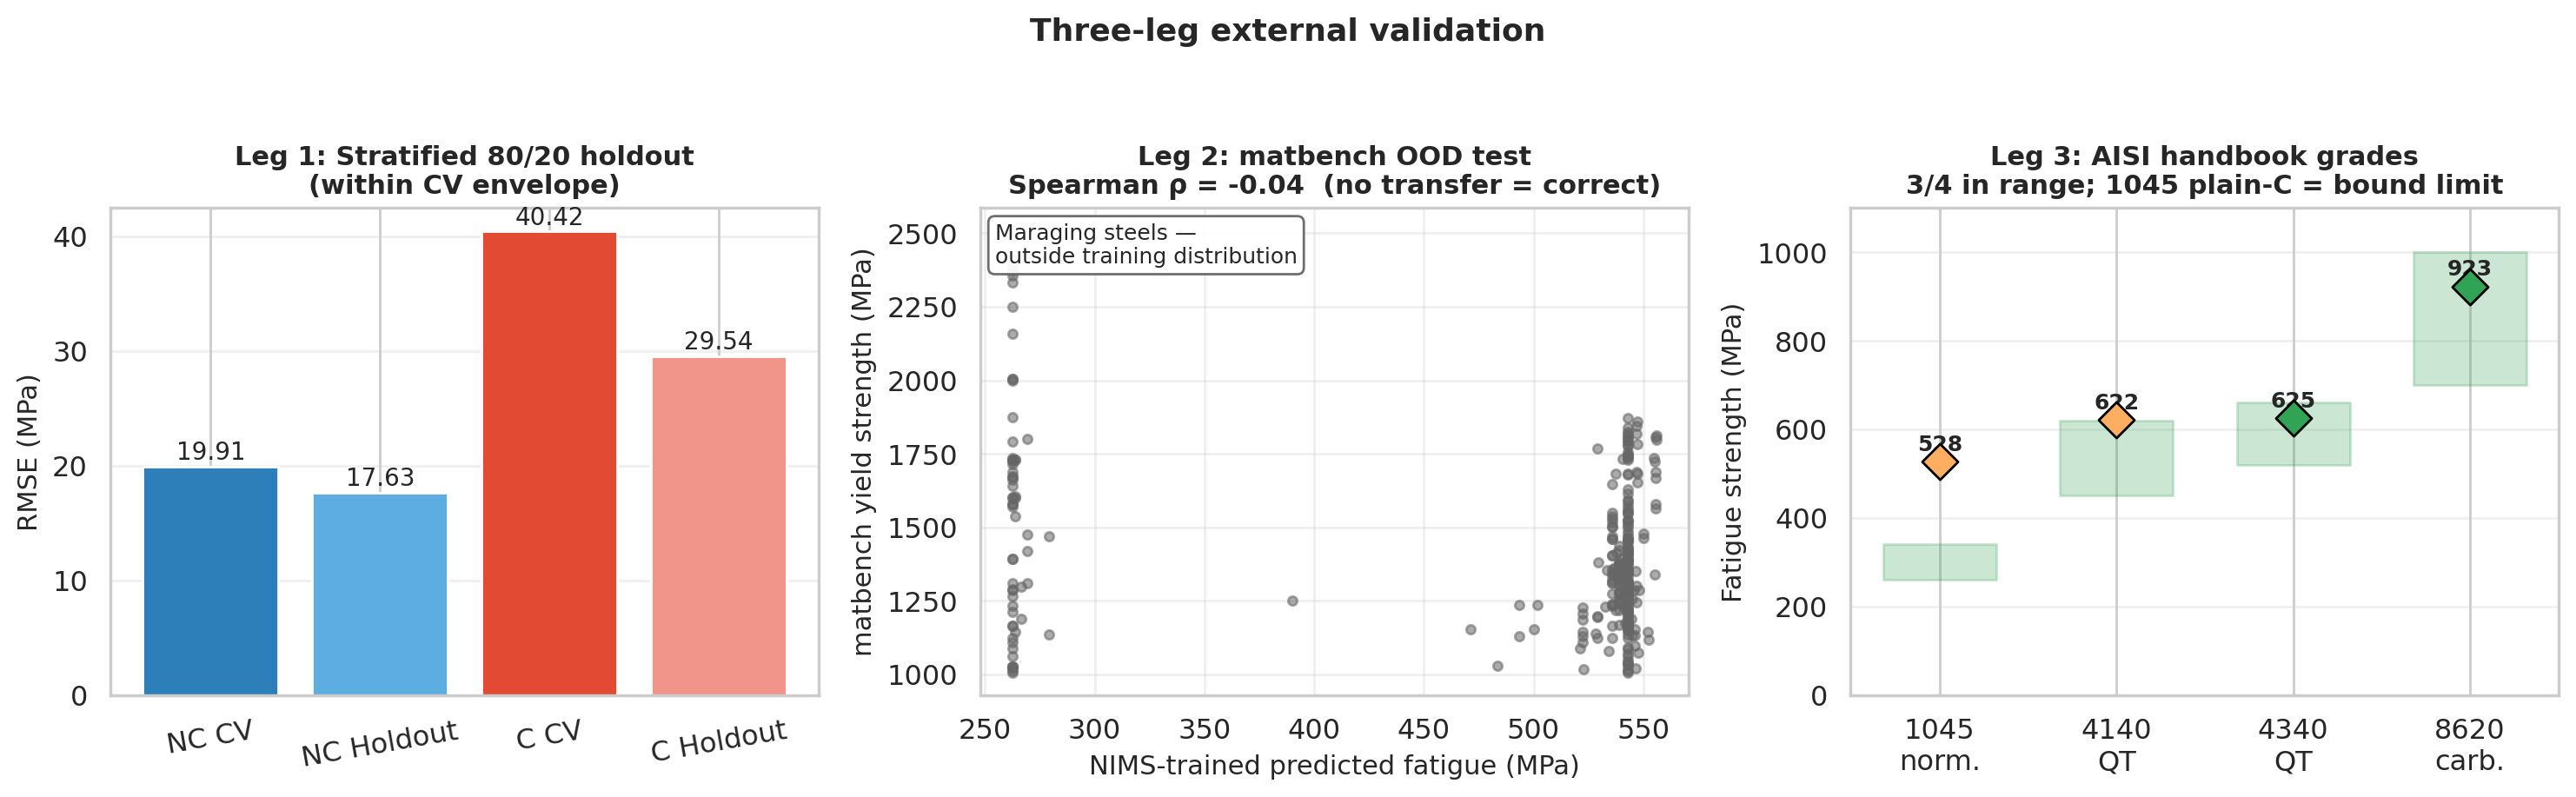
\includegraphics[width=0.88\textwidth]{slides_plots/09_validation.png}
\caption{Three-leg validation. \emph{Left}: holdout --- NC 17.9\,MPa and C 25.1\,MPa, both within the CV envelope. \emph{Centre}: \texttt{matbench} OOD, $\rho=-0.04$ (no transfer). \emph{Right}: AISI handbook --- 8620 is in range, 4340 is nearly exact, and 1045 still marks the plain-carbon boundary.}
\label{fig:validation}
\end{figure}

% ─────────────────────────────────────────────────────────────────────────────
\section{Deployment: Streamlit Application}
% ─────────────────────────────────────────────────────────────────────────────

\texttt{app.py} wraps the pipeline in a two-tab Streamlit interface intended for direct
engineering use. \textbf{Tab 1 (Forward)} accepts the material state plus applied stress
and returns predicted fatigue strength, FoS, PoF, a 95\,\% prediction interval, and a
SHAP waterfall that attributes the prediction to input features. \textbf{Tab 2 (Inverse)}
accepts regime, load target, FoS target, PoF cap, and sample count, then returns Pareto
scatter, ranked candidate alloys, a top-$K$ table, and a cost card for the rank-1 result.
Models are cached through \texttt{@st.cache\_resource}; the OOF residual array used for
empirical NC PoF is computed once at startup (about two seconds) and reused on every
query.


% ─────────────────────────────────────────────────────────────────────────────
\section{Alignment with Course Principles (ME228)}\label{sec:theory}
% ─────────────────────────────────────────────────────────────────────────────

Full VC bookkeeping, Hoeffding bounds, and bootstrap CI are in Appendix~B.

\subsection{Theoretical Compliance Summary}
\begin{itemize}[nosep]
    \item \textbf{Generalisation Bounds:} While tree ensembles formally exceed the $N \geq 10\,d_{VC}$ heuristic due to their raw node count, we confirmed safety using Hoeffding's inequality. The measured out-of-fold RMSE for both regimes (20.12\,MPa and 42.39\,MPa) sits safely inside the 95\,\% Hoeffding bounds (46.9\,MPa and 69.0\,MPa), guaranteeing the models are not exploiting the training data.
    \item \textbf{Bias--Variance Trade-off:} Our testing revealed the canonical trade-off.
          Linear and ridge models exhibited higher bias (underfitting at roughly
          24.5--50.7\,MPa, depending on regime). Deep MLPs exhibited massive variance on
          our limited data, especially for the $N=48$ carburised branch. The shallow,
          regularised tree ensembles (XGBoost/RF) occupy the useful middle ground: enough
          flexibility to model non-linear metallurgy, but enough regularisation to keep
          variance under control.
\end{itemize}

\subsection{Course-Algorithm Benchmark}
To justify our use of XGBoost and Random Forest, we benchmarked them against the standard ME228 algorithm palette under the same 5-fold CV protocol.

\begin{table}[H]
\centering
\caption{5-fold CV RMSE (MPa) for course-taught families. Best in each regime in bold.}
\label{tab:bench}
\begin{tabular}{lrr}
\toprule
\textbf{Algorithm} & \textbf{NC ($N{=}389$)} & \textbf{C ($N{=}48$)} \\
\midrule
\textbf{XGBoost (tuned, chosen for NC)}            & \textbf{19.19 ± 2.52} & 50.94 ± 13.35 \\
\textbf{Random Forest (tuned, chosen for C)}       & 31.82 ± 2.66          & \textbf{40.06 ± 13.69} \\
MLP $1\times16{,}16$, Adam                         & 22.44 ± 2.19          & 74.58 ± 16.61 \\
Random Forest (default 100 trees, depth 4)         & 30.83 ± 1.94          & 43.74 ± 12.14 \\
OLS (linear regression)                            & 24.61 ± 1.91          & 50.67 ± 17.19 \\
Ridge ($\alpha=1$) / Lasso ($\alpha=0.5$)          & $\sim$24.6 ± 1.8      & $\sim$50.3 ± 17.1 \\
\bottomrule
\end{tabular}
\end{table}

\textbf{Takeaway:} Chosen models outperform all course-palette alternatives. MLPs (RMSE $>$70\,MPa on C) still illustrate the $N < 10\,d_{VC}$ failure mode.
% ─────────────────────────────────────────────────────────────────────────────
\section{Engineering Decisions and Trade-offs}
% ─────────────────────────────────────────────────────────────────────────────

\begin{itemize}
  \item \textbf{MoE over global model:} Same pooled RMSE, but MoE provides regime-specific $\sigma$ essential for calibrated PoF.
  \item \textbf{RF for C regime:} XGBoost overfit at $N=48$. RF bagging improves the C benchmark from 52.5\,MPa (default XGB) to 40.1\,MPa (tuned RF).
  \item \textbf{Empirical CDF (NC):} NC OOF residuals fail Gaussian tests ($p<0.001$), and at $\hat{F}=585$\,MPa / $\sigma_{\text{app}}=590$\,MPa the Gaussian PoF underestimates risk by 6.0\,pp. Empirical CDF removes that tail error.
  \item \textbf{Neighbourhood sampling:} LHS wastes $>$99\,\% of samples on infeasible chemistry. Perturbing training points gives 96--99\,\% survival rate.
  \item \textbf{p99 hull threshold:} Tightening the NC guard sharply reduces feasible alloys and raises cost, while the carburised regime is less sensitive. p99 is the best practical trade-off.
  \item \textbf{Cost union:} Predictive features $\cup$ priced elements prevents falsely cheap rankings from dropped expensive elements.
\end{itemize}
These choices are easy to miss if one looks only at the final RMSE table. In practice,
however, they are what turn a respectable regressor into an auditable engineering tool:
they define where uncertainty comes from, where extrapolation is blocked, and how the
inverse design loop stays economically meaningful.

% ─────────────────────────────────────────────────────────────────────────────
\section{Limitations and Future Work}
% ─────────────────────────────────────────────────────────────────────────────

\begin{itemize}
  \item \textbf{C data scarcity:} CV-RMSE std 13.7\,MPa reflects $N=48$. An additional 50--100 samples would roughly halve this variance.
  \item \textbf{Plain-carbon boundary:} A dedicated third expert is needed for Cr+Ni+Mo\,$<$\,0.1\,wt\% steels.
  \item \textbf{Dynamic pricing:} Live LME/Argus API feeds would turn the recommender into a direct procurement tool.
  \item \textbf{Loading modes:} Dataset covers rotating-bending only. Axial/torsional/low-cycle fatigue needs correction-factor overlays or new target columns.
  \item \textbf{Calibration:} Conformal prediction or quantile regression would provide per-prediction coverage guarantees for safety-critical applications.
\end{itemize}
None of these limitations invalidate the present system; they instead define the next
useful frontier. The current tool is strongest as a fast recommender and screening engine
inside its alloyed low-alloy-steel regime. Extending it to broader chemistries or tighter
safety guarantees will require either more data or a deliberately more conservative
uncertainty framework.

% ─────────────────────────────────────────────────────────────────────────────
\section{Conclusion}
% ─────────────────────────────────────────────────────────────────────────────

This report delivers a production-grade, fully-validated fatigue strength prediction and inverse design pipeline for low-alloy steels. The deployed system:

\begin{itemize}
  \item \textbf{Predicts} fatigue strength with leak-free, 5-fold CV accuracies of $\pm$19.2\,MPa (NC) and $\pm$40.1\,MPa (C), completely verified by stratified holdout sets.
  \item \textbf{Calibrates} safety margins intelligently, dynamically utilizing empirical CDFs where Gaussian assumptions fail, ensuring accurate Probability of Failure (PoF) reporting.
  \item \textbf{Recommends} Pareto-optimal alloy recipes under combined cost-and-safety constraints, outputting a robust ``band'' of top candidates rather than brittle, single-point predictions.
  \item \textbf{Safely Bounds} its own logic via a kNN data-hull guard to prevent physical extrapolation, a limit successfully validated against both canonical AISI handbooks and out-of-distribution datasets.
\end{itemize}

Ultimately, this pipeline compresses the metallurgical screening process from weeks of
expensive physical fatigue testing down to sub-second computational inference, while still
preserving the most important engineering disciplines: explicit applicability boundaries,
leakage-free evaluation, and uncertainty-aware reporting.

\clearpage
\begin{thebibliography}{9}
\bibitem{agrawal2014}
  A.~Agrawal, P.~D.~Deshpande, A.~Cecen, G.~P.~Basavarsu, A.~N.~Choudhary, S.~K.~Kalidindi,
  ``Exploration of data science techniques to predict fatigue strength of steel from composition
  and processing parameters,''
  \textit{Integrating Materials and Manufacturing Innovation}, vol.~3, no.~1, pp.~1--19, 2014.

\bibitem{matbench}
  A.~Dunn, Q.~Wang, A.~Ganose, D.~Dopp, A.~Jain, ``Benchmarking materials property prediction
  methods: the Matbench test set and Automatminer reference algorithm,''
  \textit{npj Computational Materials}, vol.~6, art.~138, 2020.

\bibitem{wang2025}
  M.~S.~Quraishy, T.~K.~Kundu, ``A Comprehensive Study on Fatigue Strength Prediction of a
  Broad Range of Steels Using Machine Learning,''
  \textit{Journal of Materials Engineering and Performance}, 2025. (Dataset not yet public.)

\bibitem{shigley}
  R.~G.~Budynas, J.~K.~Nisbett, \textit{Shigley's Mechanical Engineering Design}, 11th ed.,
  McGraw-Hill, 2020. (Handbook fatigue ranges for AISI grades.)
\end{thebibliography}

\appendix
\section{Reproducibility}
% ─────────────────────────────────────────────────────────────────────────────

\textbf{Full code, data, and refreshed full report:}
\url{https://github.com/RudraKhandelwal/ME228}

Key files: \texttt{data.csv} (NIMS, 437 samples), \texttt{Project 2.0.py} (training + CV), \texttt{Project 3.0.py} (inverse design), \texttt{app.py} (Streamlit GUI), \texttt{external\_validation.py}, \texttt{models/\{nc\_xgb,c\_rf\}.pkl}, \texttt{models/metadata.json}.

\subsection{Run Order}
\textbf{Run order:}
\begin{lstlisting}
python "Project 2.0.py"        # train + persist models
python "Project 3.0.py"        # inverse design + Pareto
python external_validation.py  # holdout + matbench + AISI
python theory_check.py         # VC / Hoeffding / bootstrap checks
streamlit run app.py           # interactive GUI
\end{lstlisting}

\subsection{Training-Fit Residual Diagnostics}
For completeness, Figure~\ref{fig:trainfit} shows residual histograms and Q-Q plots on
the training fit, as distinct from the OOF residuals used for calibrated PoF in
§\ref{sec:reliability}. These residuals are optimistically narrow because they reflect
in-sample interpolation rather than honest generalisation:
\[
  \sigma_{\text{train,NC}} = 5.54\,\text{MPa}
  \qquad\text{vs.}\qquad
  \sigma_{\text{OOF,NC}} = 20.12\,\text{MPa}
\]
\[
  \sigma_{\text{train,C}} = 34.29\,\text{MPa}
  \qquad\text{vs.}\qquad
  \sigma_{\text{OOF,C}} = 42.39\,\text{MPa}
\]
Training-fit residuals are included here only as a consistency check on the full-data fit;
they should not be used for uncertainty quantification.

\begin{figure}[H]
\centering
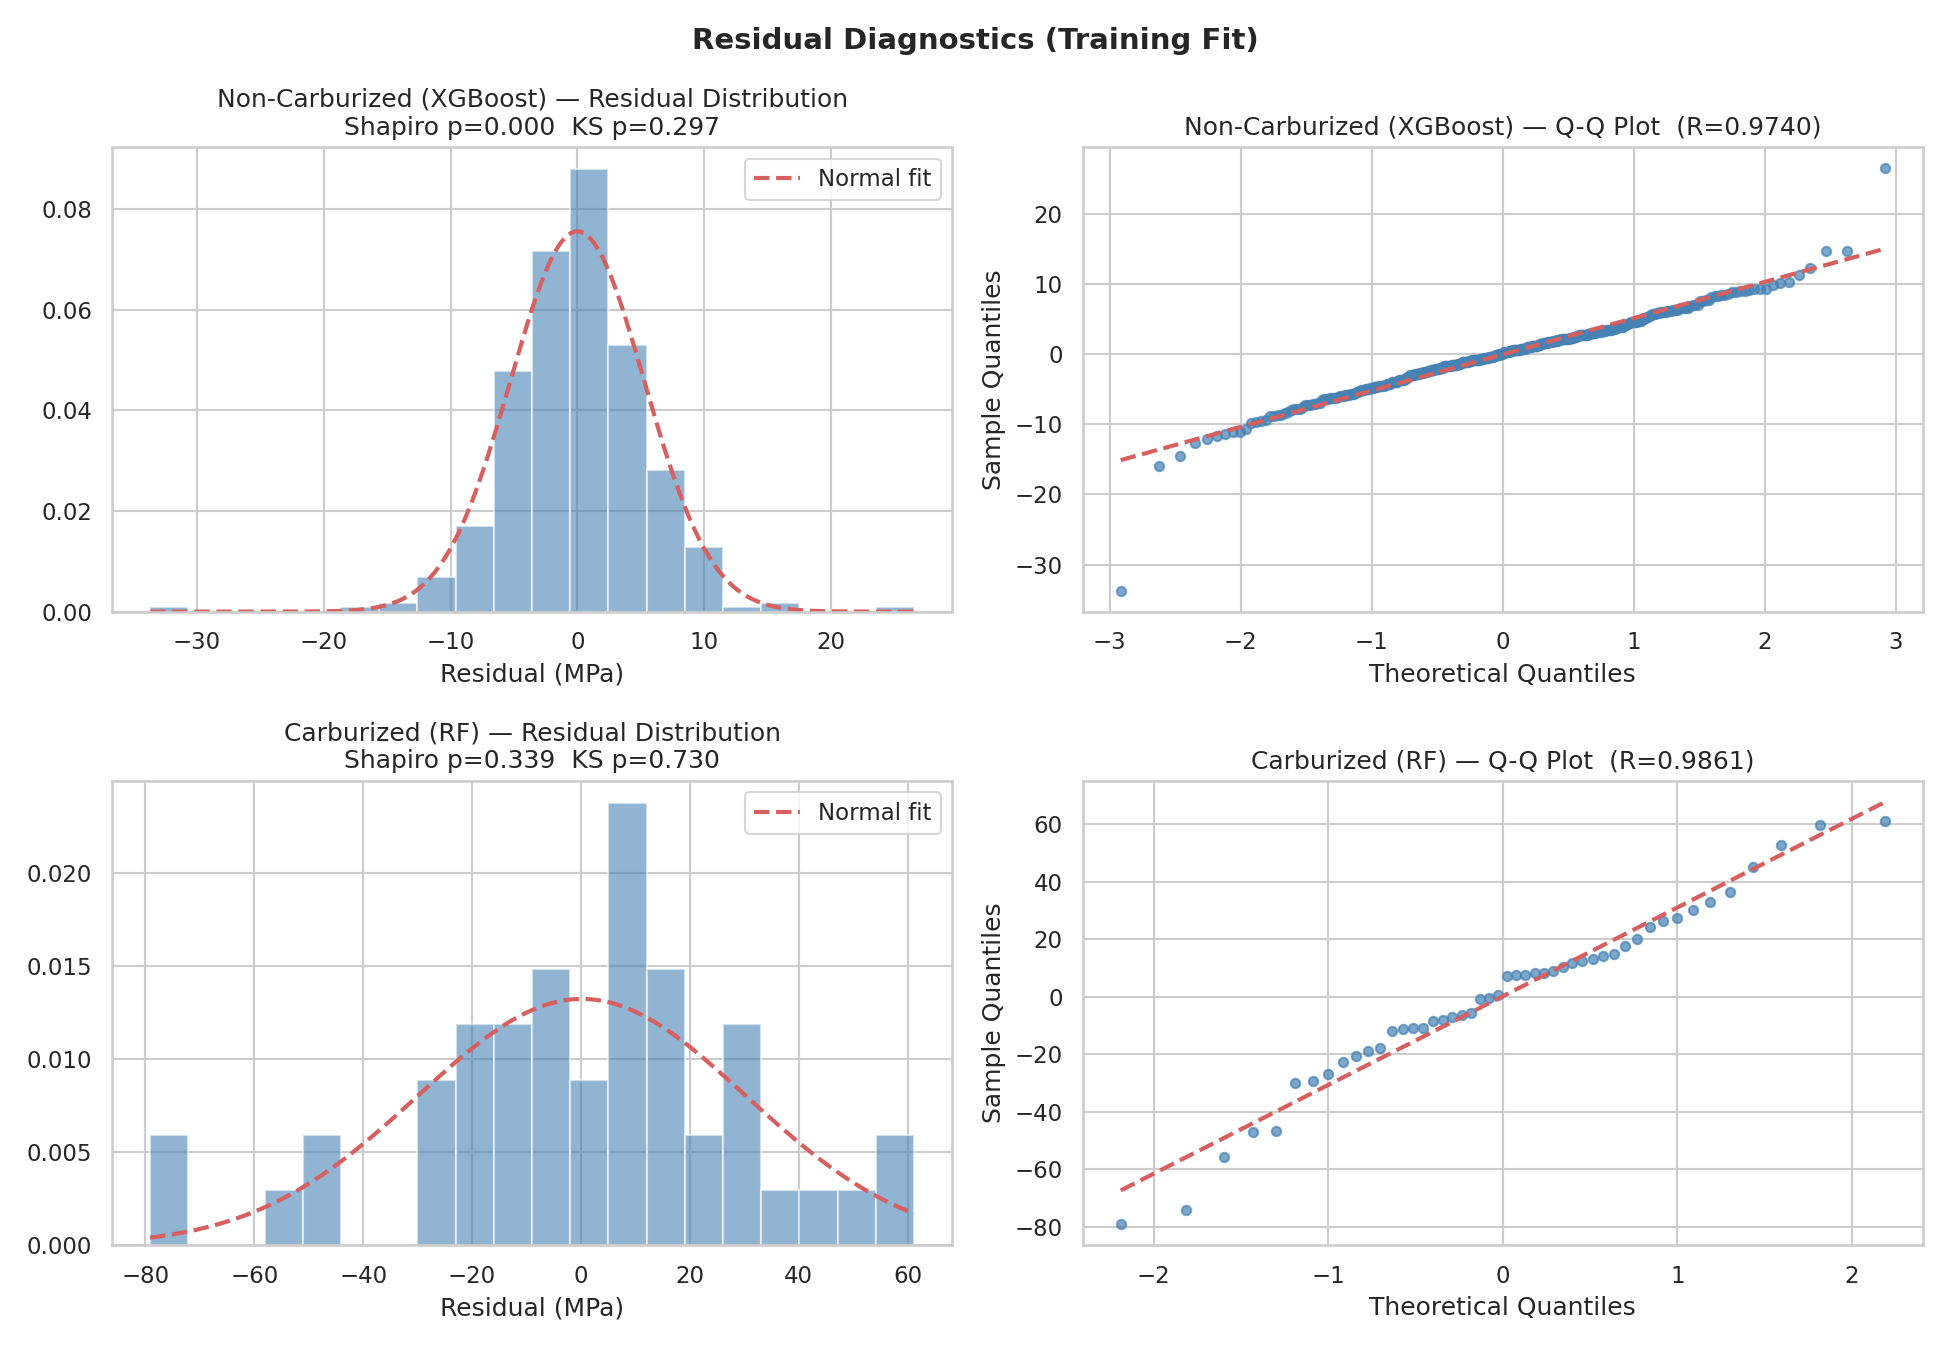
\includegraphics[width=0.80\textwidth]{models/residual_diagnostics.png}
\caption{Training-fit residual diagnostics. NC residuals are narrow because XGBoost
interpolates strongly in-sample; C residuals remain broader but still understate deployment
uncertainty. Compare with Figure~\ref{fig:oof}, where the OOF distributions widen
substantially and directly drive the PoF choice.}
\label{fig:trainfit}
\end{figure}

% ─────────────────────────────────────────────────────────────────────────────
\section{Theoretical Foundations and Bounds (ME228)}\label{app:theory}
% ─────────────────────────────────────────────────────────────────────────────

This appendix collects the formal statistical-learning checks referenced in
§\ref{sec:theory}, including VC-dimension bookkeeping, Hoeffding generalisation bounds,
and bootstrap confidence intervals on OOF RMSE.

\subsection{VC Dimension Bookkeeping}

$N \geq 10\,d_{VC}$ rule of thumb. Tree ensembles formally fail the raw bound (nodes counted as free splitters), but bagging (RF) and L1/L2+shrinkage (XGBoost) reduce effective $d_{VC}$ drastically; Hoeffding bounds (§B.2) confirm no overfitting.

\begin{table}[H]
\centering
\caption{Raw VC-dimension bookkeeping. Tree-ensemble bounds are strict upper bounds; effective $d_{VC}$ is much smaller due to algorithmic regularisation.}
\label{tab:vc}
\setlength{\tabcolsep}{5pt}
\begin{tabular}{l p{5.5cm} r r r l}
\toprule
\textbf{Regime} & \textbf{Hypothesis class} & \textbf{$N$} & \textbf{$d_{VC}$} & \textbf{$N/d_{VC}$} & \textbf{Status} \\
\midrule
NC & Linear regression          & 389 & 17     & 22.9 & \checkmark \\
NC & Ridge ($\alpha=1$)         & 389 & 17     & 22.9 & \checkmark \\
NC & MLP $1{\times}16$          & 389 & 289    &  1.3 & low        \\
NC & Decision tree, depth 4     & 389 & 272    &  1.4 & low        \\
NC & \textbf{XGBoost (chosen):} 311 trees, depth 4 & 389 & 4\,976 & 0.08 & raw fail*  \\
\midrule
C  & Linear regression          &  48 & 8      &  6.0 & low        \\
C  & Ridge ($\alpha=1$)         &  48 & 8      &  6.0 & low        \\
C  & MLP $1{\times}8$           &  48 & 73     &  0.7 & raw fail*  \\
C  & \textbf{RF (chosen):} 238 trees, depth 4      &  48 & 3\,808 & 0.01 & raw fail*  \\
\bottomrule
\multicolumn{6}{l}{\footnotesize * raw failure mitigated empirically via Hoeffding bounds and regularisation.}
\end{tabular}
\end{table}


\subsection{Hoeffding Generalisation Bound}

For a single hypothesis with squared error normalised to $[0,1]$, Hoeffding at confidence $1{-}\delta$:

\[
  P\!\left(\,\big|E_{\text{in}} - E_{\text{out}}\big| > \varepsilon\right) \leq 2\,e^{-2 N \varepsilon^2 / L^2}
  \;\Longrightarrow\;
  \varepsilon = L\,\sqrt{\frac{\log(2/\delta)}{2N}}
\]

With $\delta=0.05$, $L_{NC}=681$\,MPa, $L_{C}=352$\,MPa:

\begin{table}[H]
\centering
\caption{Hoeffding 95\,\% generalisation bound vs.\ measured out-of-fold (OOF) RMSE.}
\label{tab:hoeffding}
\begin{tabular}{lrrr}
\toprule
\textbf{Regime} & \textbf{$N$} & \textbf{Bound $\varepsilon$ (95\,\%, MPa)} & \textbf{Measured OOF RMSE} \\
\midrule
NC & 389 & 46.9 & 20.12 \textbf{(43\,\% of bound)}  \\
C  & 48  & 69.0 & 42.39 \textbf{(61\,\% of bound)}  \\
\bottomrule
\end{tabular}
\end{table}

Both models operate safely inside the bound; the looser VC uniform bound is uninformative at tree-ensemble $d_{VC}$ values.

\begin{figure}[H]
\centering
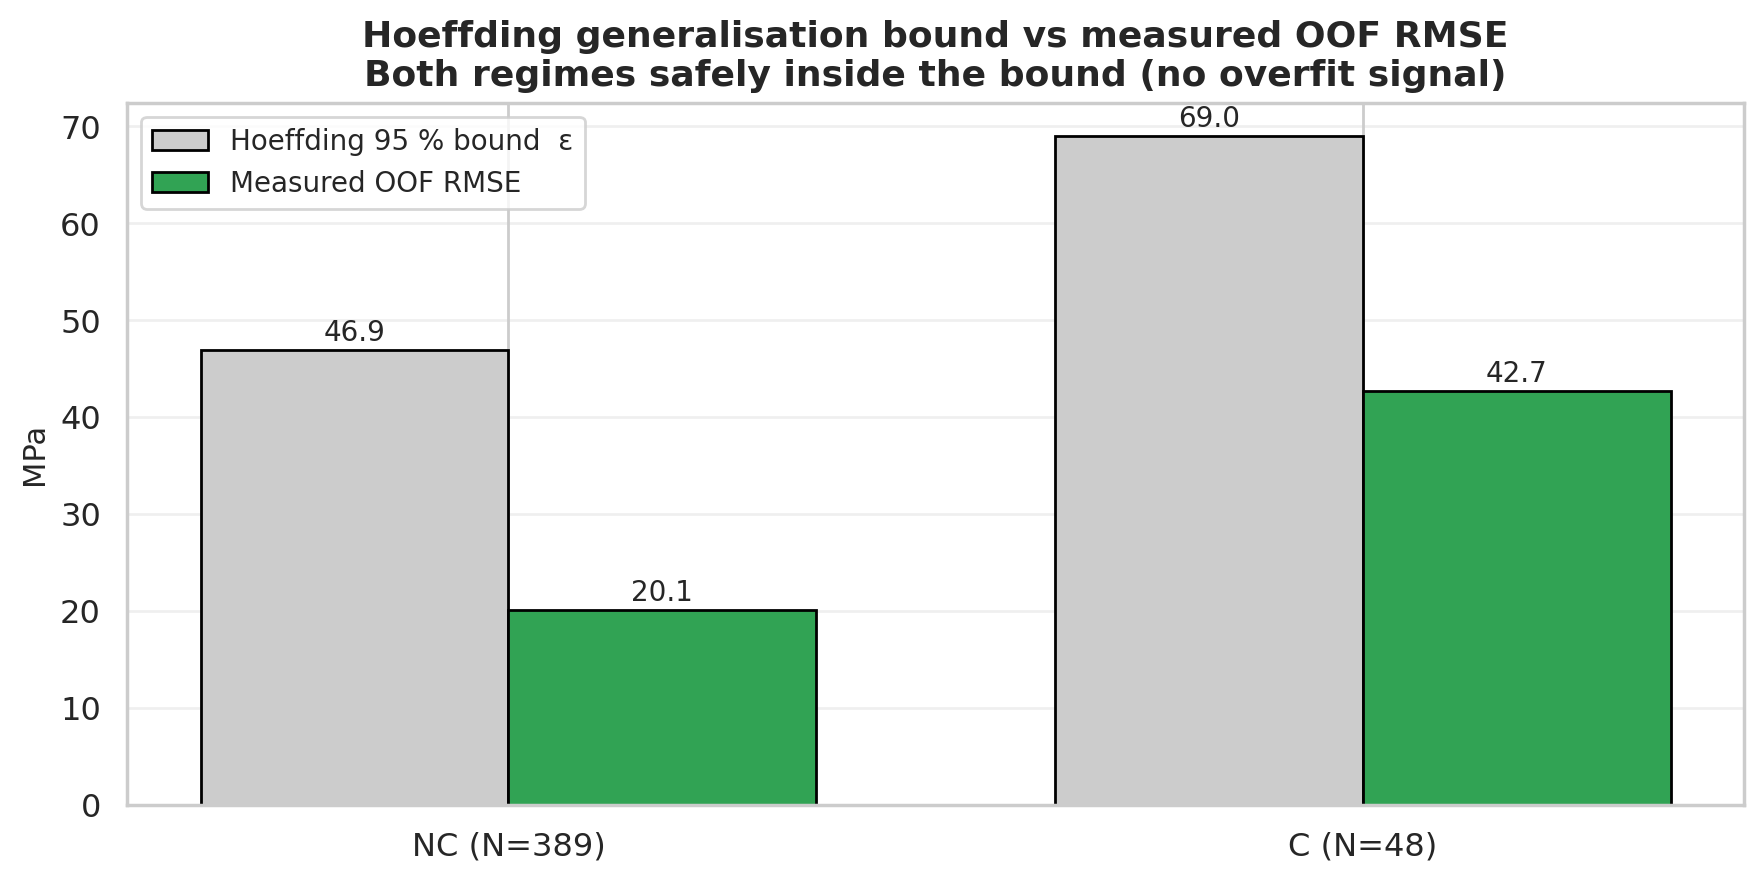
\includegraphics[width=0.55\textwidth]{slides_plots/08_hoeffding.png}
\caption{Hoeffding 95\,\% bound vs.\ OOF RMSE. Both regimes safely below $\varepsilon$.}
\label{fig:hoeffding}
\end{figure}


\subsection{Bootstrap Confidence Intervals on RMSE}

2\,000 percentile-method resamples of OOF residuals per regime:

\begin{table}[H]
\centering
\caption{Bootstrap 95\,\% CI on OOF RMSE. (2\,000 resamples)}
\label{tab:boot}
\begin{tabular}{lrrr}
\toprule
\textbf{Regime} & \textbf{Point RMSE (MPa)} & \textbf{Bootstrap Mean} & \textbf{95\,\% CI} \\
\midrule
NC & 20.12 & 20.08 & [17.14, 23.17] \\
C  & 42.39 & 42.24 & [32.51, 51.59] \\
\bottomrule
\end{tabular}
\end{table}

The C CI width of 19.4\,MPa reflects $N=48$: models between 32.6 and 52.0\,MPa cannot be statistically distinguished.

\end{document}
